% Relatório — TP "Analisando Grafos do SNAP" — G27 com-Orkut
% Todos os números vêm de valores.tex / valores_extra.tex / tabelas/ (gerados por scripts/gerar_relatorio.py).
% Comentários "% INTERPRETAÇÃO" marcam parágrafos interpretativos para a autora revisar com suas palavras.
\PassOptionsToPackage{expansion=false}{microtype}
\IfFileExists{webmedia.cls}{\documentclass[sigconf]{webmedia}}{\documentclass[sigconf]{acmart}}

\usepackage[brazilian]{babel}
\usepackage{booktabs}
\usepackage{adjustbox}
\usepackage[section]{placeins}
\usepackage{amsmath}
\usepackage{xurl}
\setlength{\emergencystretch}{2em}

\DeclareUnicodeCharacter{2260}{\ensuremath{\neq}}
\DeclareUnicodeCharacter{00B3}{\textsuperscript{3}}
\DeclareUnicodeCharacter{00B2}{\textsuperscript{2}}
\DeclareUnicodeCharacter{00B7}{\ensuremath{\cdot}}
\DeclareUnicodeCharacter{2192}{\ensuremath{\rightarrow}}
\DeclareUnicodeCharacter{2248}{\ensuremath{\approx}}
\DeclareUnicodeCharacter{2265}{\ensuremath{\geq}}
\DeclareUnicodeCharacter{2264}{\ensuremath{\leq}}
\DeclareUnicodeCharacter{2212}{\ensuremath{-}}
\DeclareUnicodeCharacter{03B3}{\ensuremath{\gamma}}
\DeclareUnicodeCharacter{03BB}{\ensuremath{\lambda}}
\DeclareUnicodeCharacter{03C3}{\ensuremath{\sigma}}
\DeclareUnicodeCharacter{03C9}{\ensuremath{\omega}}
\DeclareUnicodeCharacter{2308}{\ensuremath{\lceil}}
\DeclareUnicodeCharacter{2309}{\ensuremath{\rceil}}
\DeclareUnicodeCharacter{2229}{\ensuremath{\cap}}
\DeclareUnicodeCharacter{2079}{\textsuperscript{9}}
\DeclareUnicodeCharacter{2261}{\ensuremath{\equiv}}
\DeclareUnicodeCharacter{221A}{\ensuremath{\surd}}
\DeclareUnicodeCharacter{2208}{\ensuremath{\in}}
\DeclareUnicodeCharacter{2211}{\ensuremath{\sum}}

% Gerado automaticamente por src/relatorio.py — não editar à mão
\newcommand{\nV}{9.917}
\newcommand{\nE}{173.413}
\newcommand{\grauMin}{1}
\newcommand{\grauMax}{250}
\newcommand{\grauMedio}{34{,}97}
\newcommand{\grauMediano}{26{,}0}
\newcommand{\densidade}{0{,}00353}
\newcommand{\nComp}{1}
\newcommand{\diametro}{9}
\newcommand{\raio}{5}
\newcommand{\caminhoMedio}{3{,}764}
\newcommand{\triangulos}{1.158.975}
\newcommand{\clusterMedia}{0{,}3703}
\newcommand{\transitividade}{0{,}3276}
\newcommand{\origV}{3.072.441}
\newcommand{\origE}{117.185.083}
\newcommand{\origLacos}{0}
\newcommand{\origDuplicadas}{0}
\newcommand{\nComunidadesSel}{51}
\newcommand{\sementeComunidade}{933}
\newcommand{\eulerImpares}{4.930}
\newcommand{\nPontes}{138}
\newcommand{\nArticulacoes}{136}
\newcommand{\bfRodadas}{8}
\newcommand{\agmPeso}{1.183{,}487}
\newcommand{\tBFS}{13{,}14}
\newcommand{\tDFS}{15{,}24}
\newcommand{\tDijkstra}{62{,}81}
\newcommand{\tBellmanFord}{153{,}39}
\newcommand{\tTarjan}{31{,}84}
\newcommand{\tPrim}{263{,}18}
\newcommand{\tKruskal}{109{,}48}
\newcommand{\fwMemoriaMB}{787}
\newcommand{\fwEstimativaNumpyH}{0{,}5}
\newcommand{\fwEstimativaPythonDias}{0{,}32}
\newcommand{\swCrandER}{0{,}00352}
\newcommand{\swLrandER}{2{,}896}
\newcommand{\swSigmaER}{80{,}9}
\newcommand{\swOmegaER}{0{,}261}
\newcommand{\swCrandConf}{0{,}0108}
\newcommand{\swLrandConf}{2{,}934}
\newcommand{\swSigmaConf}{26{,}81}
\newcommand{\swOmegaConf}{0{,}271}
\newcommand{\plGammaSub}{6{,}00}
\newcommand{\plKminSub}{119}
\newcommand{\plGammaFull}{2{,}96}
\newcommand{\plKminFull}{168}
\newcommand{\plCaudaFull}{289.226}
\newcommand{\robR}{496}
\newcommand{\robSaleat}{0{,}9992}
\newcommand{\robSgrau}{0{,}9990}
\newcommand{\robSbet}{0{,}9960}
\newcommand{\robSpr}{0{,}9976}
\newcommand{\robCaleat}{7{,}8}
\newcommand{\robCgrau}{8}
\newcommand{\robCbet}{36}
\newcommand{\robLaleat}{3{,}796}
\newcommand{\robLgrau}{4{,}025}
\newcommand{\robLbet}{4{,}246}
\newcommand{\fracIntraComunidade}{87{,}4}
\newcommand{\robForaAleat}{7{,}4}
\newcommand{\robForaGrau}{9}
\newcommand{\robForaBet}{38}
\newcommand{\robForaPr}{23}
\newcommand{\sobreposicaoTopR}{147}
\newcommand{\sobreposicaoTopRPct}{30}
\newcommand{\multicomTopGrau}{73}
\newcommand{\multicomTopBet}{53}
\newcommand{\clusTopGrau}{0{,}305}
\newcommand{\clusTopBet}{0{,}195}
\newcommand{\betHubsRazao}{16}
\newcommand{\ckExpoente}{0{,}20}

% Gerado por scripts/gerar_relatorio.py
\newcommand{\cpu}{Intel(R) Xeon(R) Processor @ 2.10GHz}
\newcommand{\nucleos}{2}
\newcommand{\pyver}{3.13.18}
\newcommand{\origGrauMax}{33.313}
\newcommand{\origGrauMedio}{76{,}28}
\newcommand{\origGrauMediano}{45}
\newcommand{\origIdMax}{3.072.626}
\newcommand{\origSegLeitura}{74}
\newcommand{\indV}{9.917}
\newcommand{\indE}{173.413}
\newcommand{\grauPreservado}{40}
\newcommand{\spearmanGrauOrig}{0{,}695}
\newcommand{\desvioGrau}{30{,}86}
\newcommand{\centroTam}{1}
\newcommand{\periferiaTam}{26}
\newcommand{\paresOrdenados}{98.336.972}
\newcommand{\fracDistTres}{29{,}9}
\newcommand{\fracDistQuatro}{50{,}0}
\newcommand{\fracAteQuatro}{84{,}8}
\newcommand{\segDistancias}{13{,}4}
\newcommand{\segTriangulos}{0{,}50}
\newcommand{\wMin}{0{,}0061}
\newcommand{\wMediana}{0{,}0625}
\newcommand{\wFracUm}{3{,}5}
\newcommand{\bfsExc}{7}
\newcommand{\bfsNivelQuatro}{5.989}
\newcommand{\dfsProf}{8.043}
\newcommand{\dijDistMax}{3{,}284}
\newcommand{\dijSaltosMedios}{6{,}79}
\newcommand{\dijSaltosMax}{12}
\newcommand{\bfNegN}{1.000}
\newcommand{\bfNegRodadas}{999}
\newcommand{\pontesFolha}{134}
\newcommand{\agmFracUm}{3{,}5}
\newcommand{\tBFSMed}{13{,}14}
\newcommand{\tBFSDp}{0{,}39}
\newcommand{\tBFSInf}{13{,}00}
\newcommand{\tBFSSup}{13{,}28}
\newcommand{\rdoisBFS}{0{,}991}
\newcommand{\tDFSMed}{15{,}24}
\newcommand{\tDFSDp}{4{,}00}
\newcommand{\tDFSInf}{13{,}81}
\newcommand{\tDFSSup}{16{,}67}
\newcommand{\rdoisDFS}{0{,}976}
\newcommand{\tEulerMed}{14{,}43}
\newcommand{\tEulerDp}{0{,}49}
\newcommand{\tEulerInf}{14{,}25}
\newcommand{\tEulerSup}{14{,}61}
\newcommand{\rdoisEuler}{0{,}977}
\newcommand{\tDijkstraMed}{62{,}81}
\newcommand{\tDijkstraDp}{9{,}21}
\newcommand{\tDijkstraInf}{59{,}51}
\newcommand{\tDijkstraSup}{66{,}10}
\newcommand{\rdoisDijkstra}{0{,}998}
\newcommand{\tBellmanFordMed}{153{,}39}
\newcommand{\tBellmanFordDp}{10{,}31}
\newcommand{\tBellmanFordInf}{149{,}70}
\newcommand{\tBellmanFordSup}{157{,}08}
\newcommand{\rdoisBellmanFord}{0{,}997}
\newcommand{\tTarjanMed}{31{,}84}
\newcommand{\tTarjanDp}{2{,}25}
\newcommand{\tTarjanInf}{31{,}04}
\newcommand{\tTarjanSup}{32{,}64}
\newcommand{\rdoisTarjan}{0{,}995}
\newcommand{\tPrimMed}{263{,}18}
\newcommand{\tPrimDp}{16{,}79}
\newcommand{\tPrimInf}{257{,}17}
\newcommand{\tPrimSup}{269{,}19}
\newcommand{\rdoisPrim}{0{,}981}
\newcommand{\tKruskalMed}{109{,}48}
\newcommand{\tKruskalDp}{6{,}06}
\newcommand{\tKruskalInf}{107{,}31}
\newcommand{\tKruskalSup}{111{,}65}
\newcommand{\rdoisKruskal}{0{,}996}
\newcommand{\rdoisMin}{0{,}976}
\newcommand{\fwValN}{150}
\newcommand{\fwRdoisNumpy}{0{,}9928}
\newcommand{\fwRdoisPython}{0{,}9960}
\newcommand{\fwEstNumpyMin}{29}
\newcommand{\fwEstPythonH}{7{,}7}
\newcommand{\fwRazao}{20}
\newcommand{\fwOps}{0{,}98}
\newcommand{\swC}{0{,}3703}
\newcommand{\swL}{3{,}764}
\newcommand{\swKmedio}{34{,}97}
\newcommand{\swGammaER}{105}
\newcommand{\swLambdaER}{1{,}300}
\newcommand{\swGammaConf}{34{,}4}
\newcommand{\swLambdaConf}{1{,}283}
\newcommand{\swClatt}{0{,}728}
\newcommand{\swCrandAnal}{0{,}00353}
\newcommand{\swLrandAnal}{2{,}589}
\newcommand{\swFontes}{1.000}
\newcommand{\swTrocas}{867.065}
\newcommand{\plBrutaSub}{1{,}61}
\newcommand{\plBrutaRdoisSub}{0{,}74}
\newcommand{\plBinsSub}{0{,}94}
\newcommand{\plBinsRdoisSub}{0{,}57}
\newcommand{\plCcdfSub}{2{,}85}
\newcommand{\plCcdfRdoisSub}{0{,}74}
\newcommand{\plKsSub}{0{,}057}
\newcommand{\plErroSub}{0{,}311}
\newcommand{\plCaudaSubx}{259}
\newcommand{\plVuongSub}{-2{,}9}
\newcommand{\plKsPoissonSub}{0{,}44}
\newcommand{\plBrutaFull}{2{,}13}
\newcommand{\plBrutaRdoisFull}{0{,}84}
\newcommand{\plBinsFull}{1{,}92}
\newcommand{\plBinsRdoisFull}{0{,}89}
\newcommand{\plCcdfFull}{2{,}93}
\newcommand{\plCcdfRdoisFull}{0{,}97}
\newcommand{\plKsFull}{0{,}016}
\newcommand{\plErroFull}{0{,}004}
\newcommand{\plCaudaFullx}{289.226}
\newcommand{\plVuongFull}{33{,}9}
\newcommand{\plKsPoissonFull}{0{,}58}
\newcommand{\robCbetRazao}{4{,}6}
\newcommand{\robLbase}{3{,}778}
\newcommand{\robEbase}{0{,}280}
\newcommand{\robEaleat}{0{,}278}
\newcommand{\robEgrau}{0{,}262}
\newcommand{\robEbet}{0{,}247}
\newcommand{\robEpr}{0{,}255}
\newcommand{\robCpr}{22}
\newcommand{\robLpr}{4{,}147}
\newcommand{\robSaleatInf}{0{,}9991}
\newcommand{\robSaleatSup}{0{,}9993}
\newcommand{\robCaleatInf}{6{,}8}
\newcommand{\robCaleatSup}{8{,}9}
\newcommand{\robLaumBet}{12}
\newcommand{\robLaumGrau}{7}
\newcommand{\robLaumAleat}{0{,}5}
\newcommand{\brandesFontes}{1.000}
\newcommand{\brandesSeg}{33}
\newcommand{\brandesSpearman}{0{,}976}
\newcommand{\brandesTopCem}{87}
\newcommand{\prIter}{97}
\newcommand{\fracMultiCom}{26{,}0}
\newcommand{\spGrauBet}{0{,}65}
\newcommand{\spComBet}{0{,}24}
\newcommand{\spGrauClus}{-0{,}06}
\newcommand{\betRazaoCom}{2{,}2}
\newcommand{\ckRdois}{0{,}41}
\newcommand{\topUmPct}{9{,}4}
\newcommand{\topCincoPct}{29{,}8}
\newcommand{\baGrauMax}{568}
\newcommand{\baGamma}{2{,}93}
\newcommand{\baC}{0{,}0171}
\newcommand{\wsC}{0{,}531}
\newcommand{\wsL}{3{,}597}
\newcommand{\erGrauMax}{59}
\newcommand{\wsGrauMax}{41}
\newcommand{\razaoBFDij}{2{,}4}
\newcommand{\mnMin}{9{,}3}
\newcommand{\mnMax}{17{,}5}
\newcommand{\hubExcA}{177048}
\newcommand{\hubExcB}{24553}
\newcommand{\hubExcRazaoMin}{7}
\newcommand{\hubExcRazaoMax}{11}
\newcommand{\hubClusMin}{0{,}16}
\newcommand{\hubClusMax}{0{,}27}
\newcommand{\pontesNaoFolha}{4}


\newcommand{\autora}{Ana Beatriz Figueiredo de Aquino}
\newcommand{\matricula}{224215935}
\newcommand{\repo}{\url{https://github.com/abiaaquino/tp-grafos-snap-orkut}}
\newcommand{\instituicao}{UFBA -- Universidade Federal da Bahia}
\newcommand{\emailautora}{ana.aquino.br@gmail.com}
\newcommand{\departamento}{Instituto de Computação, Departamento de Ciência da Computação}
\newcommand{\disciplina}{MATA53-393366-2026.2 -- Teoria dos Grafos}

\settopmatter{printacmref=false}
\acmConference[MATA53 -- Teoria dos Grafos]{MATA53-393366-2026.2 -- Teoria dos Grafos -- Trabalho Prático: Analisando Grafos do SNAP}{2026.2}{UFBA, Salvador, BA, Brasil}
\setcopyright{none}
\renewcommand\footnotetextcopyrightpermission[1]{}
\pagestyle{plain}

\begin{document}

\title{Analisando Grafos do SNAP: a rede social com-Orkut (G27)}

\author{\autora}
\affiliation{\department{\departamento}\institution{\instituicao}\city{Salvador}\state{Bahia}\country{Brasil}}
\email{\emailautora}

\begin{abstract}
Este trabalho analisa o grafo G27 do SNAP, a rede social não direcionada com-Orkut (\origV{} vértices e \origE{} arestas, com comunidades \emph{ground-truth}). O arquivo bruto foi auditado em \emph{streaming} (0 auto-laços e 0 arestas duplicadas; as contagens conferem com o SNAP) e reduzido a um subgrafo induzido por \nComunidadesSel{} comunidades sobrepostas, cuja maior componente conexa tem \nV{} vértices e \nE{} arestas. Na Parte~I, o grafo tem diâmetro \diametro, raio \raio, caminho médio \caminhoMedio{} e clusterização média \clusterMedia. Na Parte~II, implementamos e validamos BFS, DFS, verificação de Euler, Dijkstra, Bellman-Ford, Floyd-Warshall, Tarjan, Prim e Kruskal, com tempos e intervalos de confiança que seguem a complexidade teórica ($R^2 \geq \rdoisMin$). Na Parte~III, a rede é \emph{small-world} mesmo contra um nulo com os mesmos graus ($\sigma = \swSigmaConf$). A lei de potência aparece no Orkut completo ($\gamma = \plGammaFull$), mas some no subgrafo amostrado. Remover os 5\% de maior grau tem o mesmo efeito que remover 5\% ao acaso, enquanto remover os 5\% de maior betweenness gera \robCbet{} componentes. A descoberta principal é que esta região da rede é sustentada pelos vértices-ponte entre comunidades, e não pelos hubs. Código e dados: \repo.
\end{abstract}

\keywords{análise de redes, redes sociais, small-world, lei de potência, robustez, algoritmos em grafos}

\maketitle

% =====================================================================
\section{Introdução}
O Orkut foi uma rede social on-line muito popular no Brasil na década de 2000. O SNAP~\cite{snapnets} disponibiliza um retrato da rede de amizades coletado por \citet{mislove2007} e organizado por \citet{yang2012} como com-Orkut: um grafo não direcionado, sem pesos, em que cada vértice é um usuário e cada aresta uma amizade. Os grupos criados pelos usuários formam as comunidades \emph{ground-truth}. O dataset é interessante por dois motivos. É uma rede social real em grande escala, com 117 milhões de arestas. E traz comunidades explícitas, o que permite relacionar estrutura local (triângulos, grupos) e estrutura global (distâncias, robustez).

O trabalho segue as três partes do enunciado. A Parte~I mede a estrutura do grafo, a Parte~II implementa e cronometra algoritmos clássicos e a Parte~III investiga propriedades de redes complexas (\emph{small-world}, lei de potência, robustez e uma descoberta). As Seções~\ref{sec:grafo}--\ref{sec:tratamento} descrevem a escolha do grafo, o código, o grafo original e o tratamento. A Seção~\ref{sec:metodo} descreve a metodologia, a Seção~\ref{sec:resultados} os resultados e a Seção~\ref{sec:discussao} as limitações.

% =====================================================================
\section{Determinação do grafo}\label{sec:grafo}
A regra do enunciado é $f(M) = (\text{soma dos dígitos de } M) \times (M \bmod 100 + 1) \bmod 129$, com $f(M) = 129$ se o resultado for 0. Para $M = \matricula$:
\begin{itemize}
\item soma dos dígitos: $2+2+4+2+1+5+9+3+5 = 33$;
\item $M \bmod 100 = 35$, logo $M \bmod 100 + 1 = 36$;
\item $33 \times 36 = 1188$ e $1188 = 9 \times 129 + 27$, logo $f(M) = 27$.
\end{itemize}
O grafo é o \textbf{G27, com-Orkut}. Na planilha de datasets, o mesmo arquivo do SNAP pode aparecer em mais de um índice ou categoria. Usamos os arquivos \texttt{com-orkut.ungraph.txt.gz} (arestas) e \texttt{com-orkut.top5000.cmty.txt.gz} (as 5.000 maiores comunidades).

% =====================================================================
\section{Código e dados}
Todo o código está em \repo. A lógica fica em \texttt{src/}, com um módulo por tema: estrutura do grafo, algoritmos, métricas, distâncias, centralidade, modelos, lei de potência, robustez, medição, figuras e formatação. O \texttt{notebook.ipynb} apenas orquestra. Os scripts são: \texttt{tratamento\_orkut.py} (auditoria e redução), \texttt{graus\_grafo\_completo.py} (distribuição de graus do Orkut inteiro), \texttt{verificar\_dados.py} (confere os dados tratados e retorna código diferente de 0 se algo divergir), \texttt{run\_all.py} (todas as análises sem o notebook) e \texttt{gerar\_relatorio.py} (gera as tabelas e macros deste texto, de modo que nenhum número foi digitado à mão). A pasta \texttt{tests/} tem 24 testes \texttt{pytest} que comparam as implementações próprias com networkx~\cite{hagberg2008} e igraph~\cite{csardi2006} em grafos pequenos com semente fixa e em casos construídos: ciclo, caminho, estrela, ciclo negativo e grafo desconexo. O README traz uma tabela que liga cada requisito do enunciado à seção do notebook, ao código e ao arquivo de saída. O arquivo bruto (448~MB) não é versionado; os dados tratados ocupam 3~MB.

% =====================================================================
\section{Descrição do grafo original}\label{sec:original}
O arquivo de arestas tem 4 linhas de comentário e uma aresta por linha (\texttt{FromNodeId}, \texttt{ToNodeId}), cada aresta não direcionada registrada uma única vez. O grafo não tem marcas de tempo, pesos nem sinais. A auditoria (Seção~\ref{sec:tratamento}) encontrou \origV{} vértices e \origE{} arestas, os mesmos valores da página do SNAP, com ids entre 1 e \origIdMax{} (há lacunas). No grafo completo, o grau médio é \origGrauMedio, o mediano \origGrauMediano{} e o máximo \origGrauMax. A distribuição de graus do grafo original aparece na linha inferior da Figura~\ref{fig:powerlaw}: cauda longa que cobre quatro ordens de grandeza. O arquivo de comunidades tem uma comunidade por linha, com tamanhos entre 3 e 4.785 membros (mediana 115). Os vértices podem pertencer a várias comunidades.

% =====================================================================
\section{Tratamento dos dados}\label{sec:tratamento}
O tratamento é feito pelo script \texttt{tratamento\_orkut.py}, que lê o \texttt{.txt.gz} uma única vez, em blocos de 5 milhões de linhas, usando menos de 1~GB de RAM (\origSegLeitura{}~s). A Tabela~\ref{tab:tratamentos} resume os passos. As decisões foram:
\begin{enumerate}
\item \textbf{Auditoria exata.} Cada aresta vira uma chave canônica $(\min(u,v), \max(u,v))$ em 64 bits, gravada em 32 arquivos temporários por \emph{hash}; cada arquivo é ordenado separadamente para contar repetições. Resultado: \origLacos{} auto-laços e \origDuplicadas{} duplicatas, inclusive no par $u$--$v$ / $v$--$u$. Todas as linhas têm $u < v$.
\item \textbf{Por que reduzir.} Com 117 milhões de arestas, as medidas exatas de distância ($O(n \cdot m)$) e o Floyd-Warshall ($O(n^3)$) são inviáveis em Python. O enunciado sugere trabalhar com alguns milhares de vértices.
\item \textbf{Como reduzir: subgrafo induzido por comunidades.} Uma semente aleatória fixa (\texttt{seed=42}) escolhe a comunidade inicial (\#\sementeComunidade). A cada passo, entra a comunidade de maior sobreposição relativa $|C \cap S|/|C|$ com o conjunto $S$ já escolhido; comunidades com mais de 2.000 membros são ignoradas. Avaliamos os prefixos da lista e escolhemos o maior cuja componente gigante tivesse no máximo 10.000 vértices: \nComunidadesSel{} comunidades. O subgrafo induzido preserva \emph{todas} as arestas do Orkut entre os vértices escolhidos, e com isso triângulos e estrutura comunitária. Uma amostragem aleatória de arestas destruiria esses padrões.
\item \textbf{Maior componente conexa.} O induzido já era conexo (\indV{} vértices, \indE{} arestas), então a LCC é o próprio induzido.
\item \textbf{Grafo simples e não direcionado.} Como não há laços nem duplicatas, nada precisou ser removido. Não existe versão dirigida a manter.
\item \textbf{Pesos.} O SNAP não fornece pesos. Usamos o peso unitário e um peso derivado dos dados, $w(u,v) = 1/(1 + |N(u) \cap N(v)|)$ (\emph{embeddedness}): laços com muitos amigos em comum ficam curtos e laços-ponte ficam longos, na linha dos laços fracos de \citet{granovetter1973}. A mediana de $w$ é \wMediana; \wFracUm\% das arestas têm $w = 1$ (nenhum amigo em comum).
\item \textbf{Graus do grafo completo.} Para testar a lei de potência sem o viés da amostra, um segundo script percorre o bruto e grava apenas a distribuição $(k, \text{nº de vértices})$ do Orkut completo (21~kB).
\end{enumerate}
O viés da redução é conhecido. A amostra fica centrada em grupos densos, e cada vértice mantém em média \grauPreservado\% do seu grau original (correlação de Spearman entre os graus: \spearmanGrauOrig). Esse efeito é discutido na Seção~\ref{sec:lp}.

\begin{table*}[!htb]
\centering
\caption{Tratamentos aplicados ao com-Orkut, com as contagens após cada passo.}
\label{tab:tratamentos}
\begin{adjustbox}{max width=\linewidth}
\begin{tabular}{p{3.2cm}p{8.6cm}p{5.2cm}}
\toprule
Tratamento & Descrição & Resultado \\
\midrule
Leitura do bruto & com-orkut.ungraph.txt.gz, leitura em streaming (blocos de 5.000.000 linhas) & 4 linhas de comentário; 117.185.083 linhas de aresta \\
Auditoria de vértices & vértices distintos que aparecem em alguma aresta & 3.072.441 (SNAP: 3.072.441; ids 1–3.072.626) \\
Auditoria de arestas & linhas de aresta vs. valor oficial & 117.185.083 (SNAP: 117.185.083) \\
Auto-laços & linhas com u = v & 0 \\
Arestas duplicadas & pares repetidos, considerando (u,v) ≡ (v,u) & 0 \\
Orientação & linhas com u > v (arquivo grava cada aresta uma vez?) & 0 \\
Seleção de comunidades & semente aleatória fixa (seed=42) + expansão gulosa por sobreposição |C∩S|/|C|; comunidades com > 2.000 nós ignoradas & semente \#933; 51 comunidades selecionadas \\
Subgrafo induzido & todas as arestas do grafo original com as duas pontas no conjunto & |V|=9.917; |E|=173.413; 1 componente \\
Simplificação & remoção de auto-laços e duplicatas; grafo não direcionado, sem pesos & 0 laços; arestas únicas por par \\
Maior componente conexa & mantida só a LCC (distâncias, diâmetro, small-world) & |V|=9.917; |E|=173.413 \\
\bottomrule
\end{tabular}
\end{adjustbox}
\end{table*}


% =====================================================================
\section{Metodologia}\label{sec:metodo}
\paragraph{Implementação e validação.} O grafo é guardado em três formas: lista de arestas, lista de adjacência e CSR. Todos os algoritmos das Partes~II e III são implementação própria, sempre validados contra uma referência independente. As bibliotecas prontas são usadas só para a BFS em C (igraph), para conferências e para o layout da visualização (networkx).

\paragraph{Distâncias.} Diâmetro, raio e caminho médio são \emph{exatos}: uma BFS a partir de cada um dos \nV{} vértices, em C (igraph), processada em blocos de 500 fontes. Assim nunca se materializa a matriz $n \times n$, que teria 750~MB. O processo leva \segDistancias~s; as excentricidades de 20 fontes foram conferidas com a nossa BFS em Python. Os triângulos são contados por orientação pelo grau, em $O(m\sqrt{m})$.

\paragraph{Medição de tempo.} Cada medição descarta 1 execução de aquecimento e desliga o coletor de lixo (\texttt{gc}). No grafo completo usamos 30 repetições e IC de 95\% Normal, $\bar{x} \pm 1{,}96\, s/\sqrt{n}$. Nos subgrafos BFS crescentes de 1.000 a \nV{} vértices (raiz aleatória fixa), usamos 10 repetições por tamanho e IC $t$-Student com 9 graus de liberdade ($t = 2{,}262$), pois $n < 30$ e $\sigma$ é desconhecido. Ajustamos $t \approx c \cdot f(n,m)$ por mínimos quadrados e reportamos o $R^2$. Ambiente: \cpu, \nucleos{} núcleos lógicos, Python \pyver.

\paragraph{Small-world.} Comparamos $C$ e $L$ do grafo com os valores médios de duas referências geradas por nós: (i) Erdős–Rényi $G(n,m)$~\cite{erdos1959} (5 instâncias) e (ii) o modelo de configuração, obtido por \swTrocas{} trocas duplas de arestas que preservam o grau de cada vértice~\cite{maslov2002} (3 instâncias). O critério de \citet{watts1998} pede $L \approx L_{\text{aleatório}}$ e $C \gg C_{\text{aleatório}}$. Calculamos $\sigma = (C/C_r)/(L/L_r)$~\cite{humphries2008} e $\omega = L_r/L - C/C_{\text{ret}}$~\cite{telesford2011}, com $C_{\text{ret}} = 3(k-2)/(4(k-1))$ para um anel regular. Declaramos \emph{small-world} se $L/L_r \leq 1{,}5$, $C/C_r \geq 10$ e $\sigma > 1$. Nenhuma função pronta de \emph{small-world} foi chamada.

\paragraph{Lei de potência.} Testamos $P(k) \sim C k^{-\gamma}$ de quatro formas: regressão em $\log P(k) \times \log k$ com pontos brutos e com bins logarítmicos; regressão na CCDF $P(K \geq k)$, cuja inclinação é $-(\gamma - 1)$; e máxima verossimilhança discreta~\cite{clauset2009}, normalizada pela zeta de Hurwitz $\zeta(\gamma, k_{\min})$, com $k_{\min}$ escolhido pela menor distância de Kolmogorov--Smirnov. A lei de potência foi comparada à exponencial na mesma cauda pelo teste de Vuong~\cite{vuong1989} e, globalmente, à Poisson que um grafo ER produziria.

\paragraph{Robustez.} Seguindo \citet{albert2000}, removemos $r = \lceil 0{,}05\,n \rceil = \robR$ vértices de duas maneiras. Na remoção aleatória, fizemos 30 repetições. Nos ataques, removemos os $r$ primeiros de um ranking fixo calculado no grafo intacto, por grau, por betweenness (Brandes~\cite{brandes2001} amostrado com \brandesFontes{} fontes e escala $n/k$~\cite{brandes2007}) ou por PageRank~\cite{page1999} (iteração de potência). As métricas são: (A) $S$, a fração dos vértices restantes na maior componente; (B) $c$, o número de componentes; (C) $L$, o caminho médio na maior componente; e (D) $E$, a eficiência global~\cite{latora2001}. $L$ e $E$ foram estimados com 200 fontes. O betweenness amostrado teve correlação de Spearman de \brandesSpearman{} com o exato do igraph, e \brandesTopCem\% de sobreposição no top-100. O nosso PageRank difere do igraph em menos de $10^{-12}$.

% =====================================================================
\section{Resultados}\label{sec:resultados}
\subsection{Parte I --- Análise estrutural}
\begin{table}[!htb]
\centering
\caption{Medidas estruturais da LCC tratada (distâncias exatas sobre todos os pares).}
\label{tab:parte1}
\begin{adjustbox}{max width=\linewidth}
\begin{tabular}{lr}
\toprule
Medida & Valor \\
\midrule
Vértices |V| & 9.917,0000 \\
Arestas |E| & 173.413,0000 \\
Grau mínimo & 1,0000 \\
Grau máximo & 250,0000 \\
Grau médio & 34,9729 \\
Grau mediano & 26,0000 \\
Densidade & 0,0035 \\
Componentes conexas & 1,0000 \\
Tamanho da maior componente & 9.917,0000 \\
Diâmetro & 9,0000 \\
Raio & 5,0000 \\
Comprimento médio dos caminhos & 3,7641 \\
Triângulos & 1.158.975,0000 \\
Clusterização média & 0,3703 \\
Transitividade (global) & 0,3276 \\
\bottomrule
\end{tabular}
\end{adjustbox}
\end{table}


\paragraph{Tamanho, graus e densidade.} A Tabela~\ref{tab:parte1} reúne as medidas. O grafo tem \nV{} vértices e \nE{} arestas. O grau vai de \grauMin{} a \grauMax, com média \grauMedio{} (desvio-padrão \desvioGrau) e mediana \grauMediano. A densidade é \densidade: o grafo é esparso, pois cada usuário se liga a menos de 0,4\% dos demais. A Figura~\ref{fig:graus} mostra a distribuição: o histograma é assimétrico à direita, o log-log tem um platô até $k \approx 20$ e depois cai cada vez mais rápido, e a CCDF despenca perto de $k = 250$. Esse corte é efeito da amostragem, discutido na Seção~\ref{sec:lp}.

\begin{figure*}[!htb]
\centering
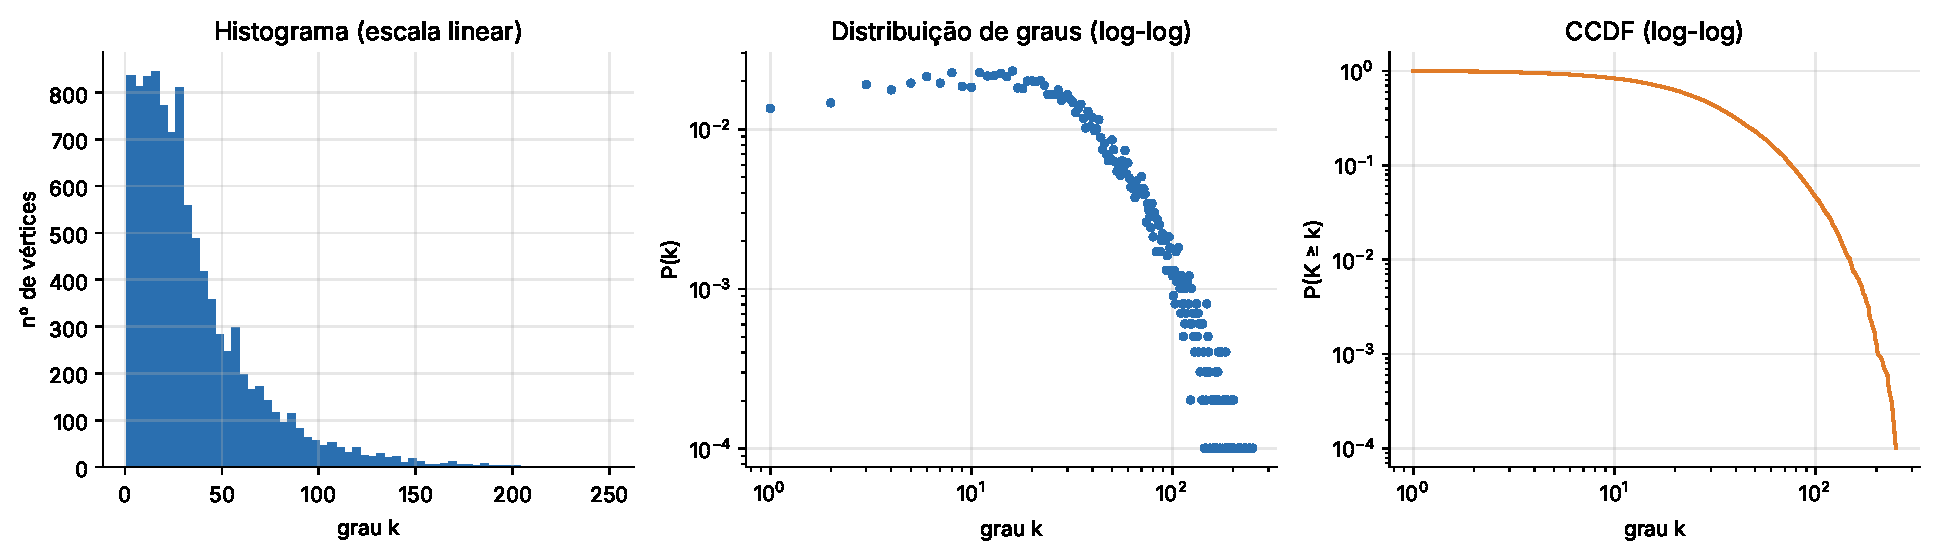
\includegraphics[width=\textwidth]{figuras/p1_distribuicao_graus.pdf}
\caption{Distribuição de graus da LCC tratada: histograma em escala linear (60 bins), $P(k)$ em log-log (vértices com $k = 0$ excluídos) e CCDF $P(K \geq k)$ em log-log.}
\label{fig:graus}
\end{figure*}

\paragraph{Componentes.} Há \nComp{} componente conexa (Tabela~\ref{tab:parte1}). Isso era esperado, porque o tratamento manteve a LCC e o induzido já era conexo.

\paragraph{Distâncias.} O diâmetro é \diametro, o raio \raio{} e o caminho médio \caminhoMedio, calculados exatamente sobre os \paresOrdenados{} pares ordenados. Só \centroTam{} vértice está no centro (excentricidade \raio) e \periferiaTam{} estão na periferia (excentricidade \diametro). A Tabela~\ref{tab:distancias} e a Figura~\ref{fig:dist} mostram que \fracAteQuatro\% dos pares estão a no máximo 4 saltos: metade (\fracDistQuatro\%) a exatamente 4 e \fracDistTres\% a 3. Em média, qualquer usuário alcança qualquer outro em menos de quatro passos.

\begin{table}[!htb]
\centering
\caption{Distribuição das distâncias (em saltos) entre os pares ordenados de vértices.}
\label{tab:distancias}
\begin{adjustbox}{max width=\linewidth}
\begin{tabular}{lrr}
\toprule
Distância & Pares ordenados & Fração (\%) \\
\midrule
1 & 346.826 & 0,35 \\
2 & 4.518.360 & 4,59 \\
3 & 29.373.624 & 29,87 \\
4 & 49.125.656 & 49,96 \\
5 & 13.757.612 & 13,99 \\
6 & 1.155.618 & 1,18 \\
7 & 57.110 & 0,06 \\
8 & 2.112 & 2,15e-3 \\
9 & 54 & 5,49e-5 \\
\bottomrule
\end{tabular}
\end{adjustbox}
\end{table}


\begin{figure}[!htb]
\centering
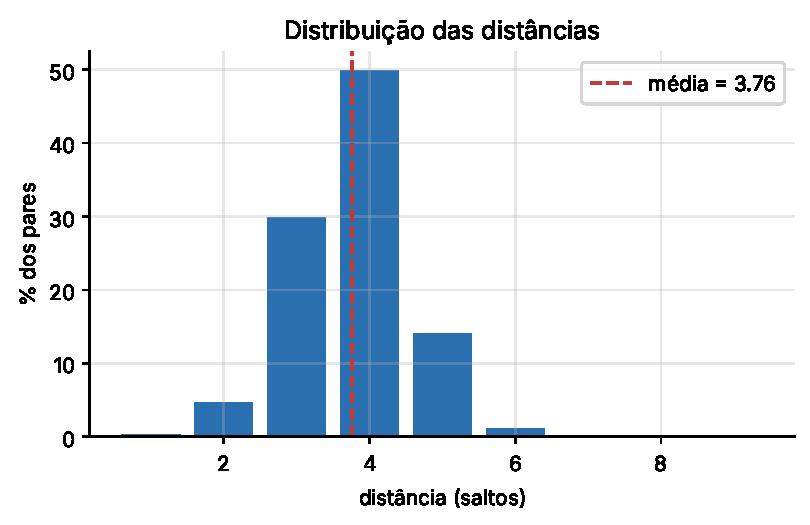
\includegraphics[width=0.85\linewidth]{figuras/p1_distribuicao_distancias.pdf}
\caption{Distribuição das distâncias (\% dos pares ordenados); a linha tracejada marca o caminho médio.}
\label{fig:dist}
\end{figure}

\paragraph{Triângulos e clusterização.} O grafo tem \triangulos{} triângulos, contados em \segTriangulos~s e conferidos com o igraph. A clusterização média é \clusterMedia{} e a transitividade global, \transitividade. Em média, 37\% dos pares de amigos de um usuário também são amigos entre si, valor cerca de cem vezes maior que a densidade.

\paragraph{Visualização.} A Figura~\ref{fig:vis} mostra os 150 vértices de maior grau (layout Kamada-Kawai), coloridos pela comunidade principal. Aparecem dois núcleos densos de comunidades sobrepostas (azul; verde/laranja/vermelho) e grupos periféricos (marrom e cinza no topo) ligados por poucas arestas. Essa imagem antecipa o papel dos vértices-ponte na Parte~III. % INTERPRETAÇÃO

\begin{figure}[!htb]
\centering
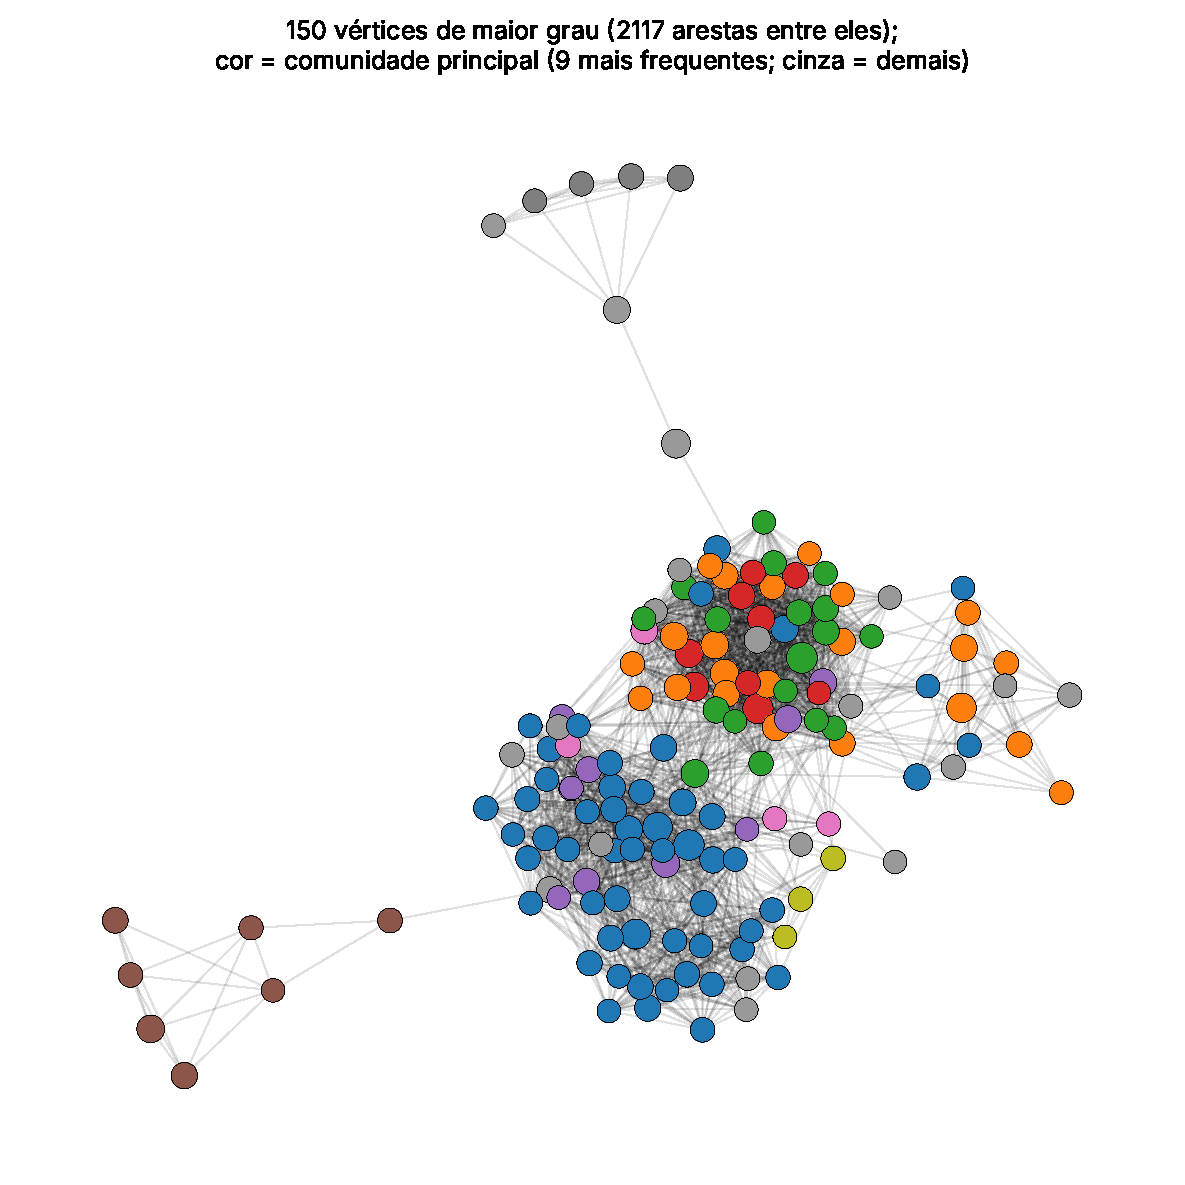
\includegraphics[width=\linewidth]{figuras/p1_visualizacao_top150.pdf}
\caption{Subgrafo dos 150 vértices de maior grau. Tamanho $\propto$ grau; cor = comunidade principal (as 9 mais frequentes; cinza = demais).}
\label{fig:vis}
\end{figure}

\paragraph{Medidas calculadas.} A Tabela~\ref{tab:calculadas} lista o método de cada medida e justifica as ausências. As medidas dirigidas (SCC, Euler dirigido) não se aplicam, porque o grafo é não direcionado. O Floyd-Warshall no grafo inteiro foi substituído por subgrafos e por extrapolação (Seção~\ref{sec:fw}). Não há pesos reais.

\begin{table*}[!htb]
\centering
\caption{Medidas calculadas e não calculadas, com o método ou a justificativa.}
\label{tab:calculadas}
\begin{adjustbox}{max width=\linewidth}
\begin{tabular}{p{4.6cm}cp{11cm}}
\toprule
Medida & Calculada & Método / justificativa \\
\midrule
Vértices e arestas & sim & contagem direta da lista de arestas \\
Grau mín./máx./médio/mediano & sim & vetor de graus (CSR) \\
Distribuição de graus & sim & histograma log-log e CCDF (k = 0 excluído) \\
Densidade & sim & 2m / (n(n-1)) \\
Componentes conexas e tamanhos & sim & BFS própria \\
Diâmetro, raio, caminho médio & sim & exato: BFS de todos os vértices (igraph, C), em blocos; conferido com BFS própria \\
Triângulos & sim & implementação própria, orientação por grau O(m·√m); conferida com igraph \\
Clusterização média e transitividade & sim & a partir dos triângulos por vértice \\
Visualização reduzida & sim & 150 vértices de maior grau, layout Kamada-Kawai \\
Componentes fortemente conexas / Euler dirigido & não & não se aplica: com-Orkut é não direcionado \\
Floyd-Warshall no grafo inteiro & não & O(n³) ≈ 9,8e11 passos e matriz de 787 MB; rodado só em subgrafos \\
Pesos reais nas arestas & não & o SNAP não fornece pesos; usamos peso unitário e um peso derivado (vizinhos em comum) \\
\bottomrule
\end{tabular}
\end{adjustbox}
\end{table*}


\subsection{Parte II --- Algoritmos}\label{sec:parte2}
A Tabela~\ref{tab:tempos} traz o tempo de cada algoritmo no grafo completo, a Tabela~\ref{tab:escala} o tempo nos subgrafos e a Tabela~\ref{tab:ajustes} o ajuste à complexidade teórica, visualizado na Figura~\ref{fig:escala}. A fonte das buscas é o vértice 0.

\begin{table*}[!htb]
\centering
\caption{Tempo no grafo completo (n = 9.917, m = 173.413): 30 repetições após 1 aquecimento, IC de 95\% Normal (z = 1,96).}
\label{tab:tempos}
\begin{adjustbox}{max width=\linewidth}
\begin{tabular}{llrrrrl}
\toprule
Algoritmo & Complexidade & Média (ms) & DP (ms) & IC95 inf. (ms) & IC95 sup. (ms) & Método do IC \\
\midrule
BFS & O(n+m) & 13,14 & 0,39 & 13,00 & 13,28 & z \\
DFS & O(n+m) & 15,24 & 4,00 & 13,81 & 16,67 & z \\
Euler (verificação) & O(n+m) & 14,43 & 0,49 & 14,25 & 14,61 & z \\
Dijkstra & O((n+m) log n) & 62,81 & 9,21 & 59,51 & 66,10 & z \\
Bellman-Ford & O(n·m) [efetivo O(k·m)] & 153,39 & 10,31 & 149,70 & 157,08 & z \\
Tarjan (pontes/articulações) & O(n+m) & 31,84 & 2,25 & 31,04 & 32,64 & z \\
Prim & O(m log n) & 263,18 & 16,79 & 257,17 & 269,19 & z \\
Kruskal & O(m log m) & 109,48 & 6,06 & 107,31 & 111,65 & z \\
\bottomrule
\end{tabular}
\end{adjustbox}
\end{table*}


\paragraph{BFS --- $O(n+m)$.} A BFS alcança os \nV{} vértices; a excentricidade da fonte é \bfsExc{} e o nível mais populoso é o 4 (\bfsNivelQuatro{} vértices). As distâncias coincidem com as do igraph. Tempo: \tBFSMed~ms (IC95 [\tBFSInf; \tBFSSup]~ms).

\paragraph{DFS --- $O(n+m)$.} A DFS iterativa (pilha explícita, para não estourar a recursão) também alcança todos os vértices. A árvore de busca tem profundidade \dfsProf: a DFS segue caminhos longos e quase não volta, ao contrário da BFS, cuja árvore tem profundidade \bfsExc. Tempo: \tDFSMed~ms (IC95 [\tDFSInf; \tDFSSup]~ms).

\paragraph{Euler --- $O(n+m)$.} Um grafo não direcionado conexo é euleriano se todos os graus são pares, e semi-euleriano se exatamente dois são ímpares. Aqui \eulerImpares{} vértices têm grau ímpar, então o grafo \textbf{não é euleriano nem semi-euleriano}. O algoritmo de Hierholzer, implementado para os casos positivos, foi validado nos testes (circuito em $K_5$). Tempo da verificação: \tEulerMed~ms.

\paragraph{Dijkstra --- $O((n+m)\log n)$.} Com peso unitário, o Dijkstra com heap binário reproduz exatamente as distâncias da BFS (validação). Com o peso de \emph{embeddedness}, a maior distância a partir da fonte é \dijDistMax. Os caminhos mínimos ponderados têm em média \dijSaltosMedios{} saltos (máximo \dijSaltosMax): preferem várias arestas fortes a poucas arestas-ponte, o que confirma que o peso muda a geometria da rede. Tempo: \tDijkstraMed~ms (IC95 [\tDijkstraInf; \tDijkstraSup]~ms).

\paragraph{Bellman-Ford --- $O(n \cdot m)$.} Com os mesmos pesos, o resultado é idêntico ao Dijkstra. Graças à parada antecipada, o algoritmo convergiu em \bfRodadas{} rodadas, contra $n - 1 = 9.916$ no pior caso, então o custo efetivo é $O(k \cdot m)$ com $k = \bfRodadas$. A aplicabilidade é limitada: como todos os pesos são positivos, o Dijkstra basta. Num grafo não direcionado, uma única aresta negativa já forma um ciclo negativo ($u \to v \to u$). Para demonstrar, atribuímos $-0{,}5$ a uma aresta de um subgrafo com \bfNegN{} vértices: o algoritmo executou as \bfNegRodadas{} rodadas e detectou o ciclo. Tempo no grafo completo: \tBellmanFordMed~ms, 2,6 vezes o do Dijkstra.

\paragraph{Floyd-Warshall --- $O(n^3)$.}\label{sec:fw} No grafo completo seriam $\approx \fwOps \times 10^{12}$ atualizações e uma matriz de \fwMemoriaMB~MB, por isso rodamos o algoritmo em subgrafos BFS (Tabela~\ref{tab:floyd}, Figura~\ref{fig:fw}). Implementamos duas versões: uma vetorizada em numpy, com $n$ atualizações $O(n^2)$ feitas em C, e uma em Python puro, com três laços. Num subgrafo de \fwValN{} vértices, as duas coincidem com o Dijkstra executado a partir de todas as fontes. O ajuste $c\,n^3$ tem $R^2 = \fwRdoisNumpy$ (numpy) e \fwRdoisPython{} (Python). Para $n = 200$, a versão pura é \fwRazao{} vezes mais lenta. Extrapolando para $n = \nV$, a versão numpy levaria $\approx$ \fwEstNumpyMin~min e a versão pura $\approx$ \fwEstPythonH~h, além dos 750~MB de memória. Para todos os pares, $n$ execuções de Dijkstra ou BFS saem muito mais baratas num grafo esparso.

\begin{table}[!htb]
\centering
\caption{Floyd-Warshall em subgrafos BFS (pesos de \emph{embeddedness}); 10 repetições, IC de 95\% t-Student.}
\label{tab:floyd}
\begin{adjustbox}{max width=\linewidth}
\begin{tabular}{lrrrrrr}
\toprule
Versão & n & m & Média (ms) & DP (ms) & IC95 inf. (ms) & IC95 sup. (ms) \\
\midrule
(numpy) & 200 & 965 & 10,3 & 0,5 & 9,9 & 10,7 \\
(numpy) & 400 & 3.503 & 101,6 & 8,2 & 95,7 & 107,5 \\
(numpy) & 600 & 4.936 & 389,2 & 9,8 & 382,2 & 396,3 \\
(numpy) & 800 & 6.637 & 909,5 & 43,9 & 878,1 & 940,9 \\
(numpy) & 1.000 & 9.305 & 1.565,4 & 46,9 & 1.531,8 & 1.598,9 \\
(numpy) & 1.200 & 11.807 & 3.156,6 & 177,3 & 3.029,8 & 3.283,4 \\
(Python) & 50 & 201 & 3,8 & 0,2 & 3,7 & 3,9 \\
(Python) & 100 & 426 & 25,6 & 1,1 & 24,8 & 26,3 \\
(Python) & 150 & 685 & 90,1 & 6,1 & 85,7 & 94,5 \\
(Python) & 200 & 965 & 206,9 & 3,8 & 204,2 & 209,6 \\
(Python) & 250 & 1.304 & 453,2 & 16,6 & 441,4 & 465,1 \\
\bottomrule
\end{tabular}
\end{adjustbox}
\end{table}


\paragraph{Tarjan --- $O(n+m)$.} A versão iterativa do algoritmo de low-link~\cite{tarjan1972} encontrou \nPontes{} pontes e \nArticulacoes{} pontos de articulação, os mesmos conjuntos que o networkx. Das pontes, \pontesFolha{} ligam um vértice de grau 1 ao resto, de modo que a rede quase não tem pontes "estruturais": é 2-conexa no núcleo. Tempo: \tTarjanMed~ms.

\paragraph{Prim e Kruskal --- $O(m \log n)$ e $O(m \log m)$.} Com o peso de \emph{embeddedness}, Prim (heap, versão \emph{lazy}) e Kruskal (união-busca com compressão de caminho e união por posto) produzem árvores geradoras mínimas de mesmo peso total, \agmPeso, igual ao do igraph, com \nV{} $-$ 1 arestas. Só \agmFracUm\% das arestas da árvore têm peso 1: a árvore usa os laços fortes sempre que pode. Tempos: Prim \tPrimMed~ms e Kruskal \tKruskalMed~ms. O Prim fica mais lento porque faz um \texttt{heappush} por aresta examinada, enquanto o Kruskal faz uma única ordenação, em C.

\begin{table*}[!htb]
\centering
\caption{Tempo médio (ms) em subgrafos BFS crescentes; 10 repetições por tamanho. Os desvios-padrão e os IC de 95\% (t-Student, 9 g.l.) estão em \texttt{resultados/parte2\_tempos\_escala.csv}.}
\label{tab:escala}
\begin{adjustbox}{max width=\linewidth}
\begin{tabular}{lrrrrrrrrr}
\toprule
n & m & BFS & DFS & Euler & Dijkstra & Bellman-Ford & Tarjan & Prim & Kruskal \\
\midrule
1.000 & 9.305 & 0,88 & 0,92 & 1,05 & 2,62 & 6,54 & 2,39 & 7,26 & 4,66 \\
2.000 & 24.175 & 2,03 & 2,01 & 2,22 & 5,88 & 19,11 & 4,51 & 17,90 & 12,24 \\
4.000 & 60.968 & 5,02 & 4,98 & 5,45 & 15,46 & 56,26 & 10,89 & 57,52 & 34,62 \\
6.000 & 97.680 & 8,19 & 8,33 & 9,52 & 28,49 & 84,94 & 19,39 & 110,89 & 57,94 \\
8.000 & 138.608 & 13,41 & 12,33 & 13,73 & 39,81 & 126,07 & 29,00 & 200,43 & 79,31 \\
9.917 & 173.413 & 16,38 & 18,06 & 20,19 & 53,44 & 148,40 & 36,32 & 235,52 & 109,86 \\
\bottomrule
\end{tabular}
\end{adjustbox}
\end{table*}

\begin{table}[!htb]
\centering
\caption{Ajuste de mínimos quadrados $t \approx c\cdot f(n,m)$ aos tempos médios da Tabela~\ref{tab:escala} ($t$ em ms) e ajuste alternativo $t \approx a n + b m$.}
\label{tab:ajustes}
\begin{adjustbox}{max width=\linewidth}
\begin{tabular}{llrrr}
\toprule
Algoritmo & f(n,m) & c & R² (c·f) & R² (a·n+b·m) \\
\midrule
BFS & O(n+m) & 0,000088 & 0,9910 & 0,9952 \\
DFS & O(n+m) & 0,000090 & 0,9764 & 0,9832 \\
Euler (verificação) & O(n+m) & 0,000101 & 0,9767 & 0,9834 \\
Dijkstra & O((n+m) log n) & 0,000022 & 0,9978 & 0,9960 \\
Bellman-Ford & O(n·m) [efetivo O(k·m)] & 0,000054 & 0,9968 & 0,9970 \\
Tarjan (pontes/articulações) & O(n+m) & 0,000194 & 0,9948 & 0,9970 \\
Prim & O(m log n) & 0,000102 & 0,9810 & 0,9898 \\
Kruskal & O(m log m) & 0,000035 & 0,9963 & 0,9949 \\
\bottomrule
\end{tabular}
\end{adjustbox}
\end{table}


\begin{figure*}[!htb]
\centering
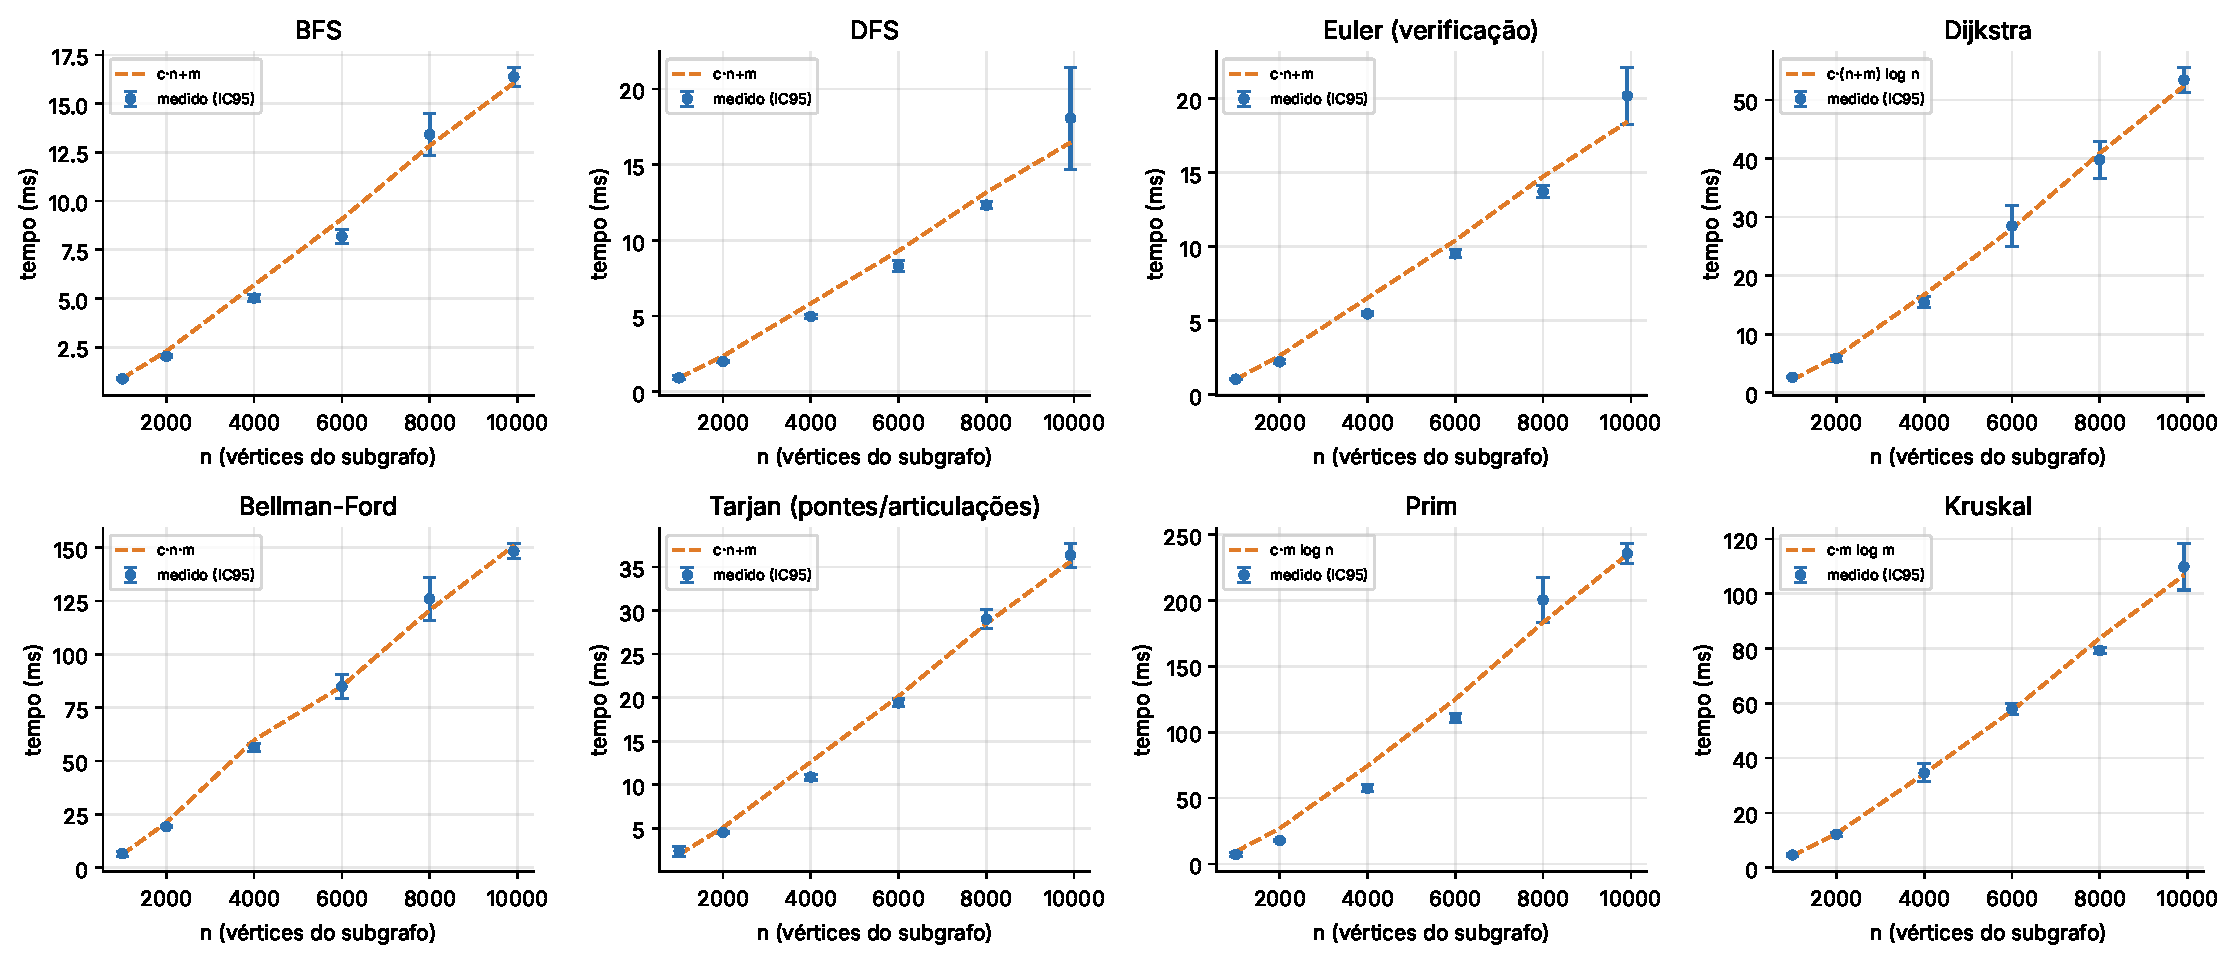
\includegraphics[width=\textwidth]{figuras/p2_escala_tempos.pdf}
\caption{Tempo médio (ms, barras = IC de 95\% t-Student, 10 repetições) em função do número de vértices dos subgrafos BFS; tracejado: ajuste $c \cdot f(n,m)$ da Tabela~\ref{tab:ajustes}.}
\label{fig:escala}
\end{figure*}

\begin{figure}[!htb]
\centering
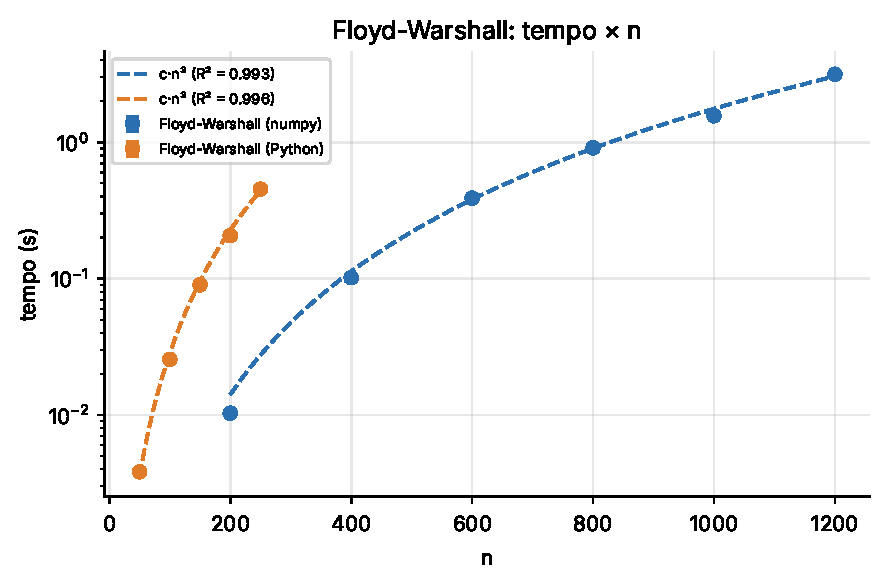
\includegraphics[width=0.9\linewidth]{figuras/p2_floyd_warshall.pdf}
\caption{Floyd-Warshall: tempo (s, escala log) $\times$ $n$ para as versões numpy e Python puro, com ajustes $c\,n^3$.}
\label{fig:fw}
\end{figure}

\paragraph{Complexidade observada.} Todos os ajustes da Tabela~\ref{tab:ajustes} têm $R^2 \geq \rdoisMin$: os tempos crescem como a complexidade teórica prevê. Há três desvios a explicar. (i) A razão $m/n$ cresce de 9,3 para 17,5 entre os subgrafos, então medir só em função de $n$ superestimaria a curvatura; por isso o eixo teórico usa $f(n,m)$. No ajuste $an + bm$, o coeficiente de $n$ sai próximo de zero, ou seja, o custo é dominado pelas arestas. (ii) No Bellman-Ford, usamos $f = k \cdot 2m$, com o número de rodadas medido em cada subgrafo; com $f = n \cdot m$, o ajuste não teria sentido. (iii) Em Python puro, a constante por operação é alta (cerca de $10^{-4}$~ms por vértice + aresta na BFS), então mesmo algoritmos lineares levam dezenas de milissegundos. A ordem relativa é coerente com a teoria: BFS $\approx$ DFS $\approx$ Euler $<$ Tarjan $<$ Dijkstra $<$ Kruskal $<$ Bellman-Ford $<$ Prim. % INTERPRETAÇÃO (iii)

\subsection{Parte III --- Redes complexas}
\subsubsection{A rede é small-world?}
\textbf{Sim.} A Tabela~\ref{tab:smallworld} e a Figura~\ref{fig:sw} mostram que o caminho médio do Orkut ($L = \swL$) é só \swLambdaER{} vezes o de um $G(n,m)$ com os mesmos $n$ e $m$ ($L_r = \swLrandER$). Já a clusterização ($C = \swC$) é \swGammaER{} vezes maior ($C_r = \swCrandER$, próximo do valor analítico $\langle k \rangle/n = \swCrandAnal$). Resulta $\sigma = \swSigmaER \gg 1$. O teste mais exigente é contra o modelo de configuração, que preserva os graus e, portanto, os hubs. Mesmo assim, $C$ continua \swGammaConf{} vezes maior ($C_r = \swCrandConf$) e $L/L_r = \swLambdaConf$, com $\sigma = \swSigmaConf$. Os dois nulos levam à mesma conclusão, mas com magnitudes diferentes: a heterogeneidade dos graus triplica a clusterização esperada ($C_{\text{conf}} \approx 3\,C_{\text{ER}}$), mas o valor ainda fica \swGammaConf{} vezes abaixo do observado. Esse restante vem da estrutura comunitária, que nenhum dos nulos reproduz. O valor $\omega = \swOmegaConf$, ligeiramente positivo, indica que a rede está mais perto do lado aleatório (caminhos curtos) do que do reticulado ($C_{\text{ret}} = \swClatt$). Na prática, a informação se espalha em poucos passos entre grupos, enquanto cada grupo permanece coeso. % INTERPRETAÇÃO

\begin{table*}[!htb]
\centering
\caption{Small-world: grafo observado contra as duas referências aleatórias (5 instâncias ER e 3 de configuração; $L_{\text{ref}}$ estimado com 1.000 fontes por instância).}
\label{tab:smallworld}
\begin{adjustbox}{max width=\linewidth}
\begin{tabular}{lrrrrrrrrr}
\toprule
Referência & C & C\_ref & C/C\_ref & L & L\_ref & L/L\_ref & σ & ω & Small-world? \\
\midrule
Erdős–Rényi G(n,m) & 0,3703 & 0,0035 & 105,1 & 3,764 & 2,896 & 1,300 & 80,9 & 0,261 & sim \\
Configuração (mesmos graus) & 0,3703 & 0,0108 & 34,4 & 3,764 & 2,934 & 1,283 & 26,8 & 0,271 & sim \\
\bottomrule
\end{tabular}
\end{adjustbox}
\end{table*}


\begin{figure}[!htb]
\centering
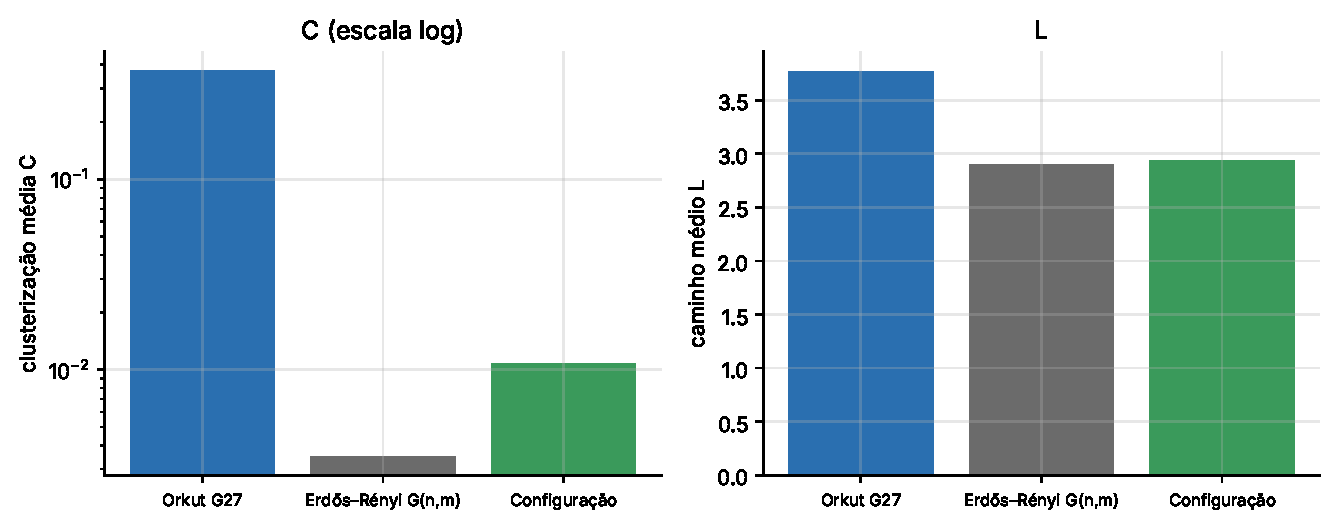
\includegraphics[width=\linewidth]{figuras/p3_small_world.pdf}
\caption{Clusterização média (escala log) e caminho médio do Orkut G27 e das referências ER e de configuração (média das instâncias).}
\label{fig:sw}
\end{figure}

\subsubsection{A distribuição de graus segue lei de potência?}\label{sec:lp}
\textbf{No Orkut completo, sim, na cauda. No subgrafo amostrado, não.} A Tabela~\ref{tab:powerlaw} e a Figura~\ref{fig:powerlaw} trazem os resultados. No grafo completo, a MLE dá $\gamma = \plGammaFull \pm \plErroFull$ para $k \geq \plKminFull$ (\plCaudaFull{} vértices na cauda, KS $= \plKsFull$). A regressão na CCDF chega a um valor quase igual (\plCcdfFull, $R^2 = \plCcdfRdoisFull$), e a lei de potência vence a exponencial com folga (Vuong $z = \plVuongFull$). A CCDF é aproximadamente reta por mais de duas décadas, de $k \approx 170$ a $k \approx 30.000$. As regressões em $P(k)$ dão valores menores (bruta \plBrutaFull; bins \plBinsFull) porque incluem o platô de graus baixos ($k < 100$), onde a lei de potência não vale; isso ilustra por que a regressão log-log isolada não é confiável~\cite{clauset2009}.

No subgrafo, os métodos divergem entre si: a regressão bruta dá \plBrutaSub, a de bins \plBinsSub{} ($R^2 = \plBinsRdoisSub$) e a MLE \plGammaSub{} numa cauda de só \plCaudaSubx{} vértices. O teste de Vuong favorece a \emph{exponencial} ($z = \plVuongSub$). A Poisson, porém, também é rejeitada (KS $= \plKsPoissonSub$): a distribuição é heterogênea, mas com a cauda cortada. A Figura~\ref{fig:grauorig} mostra a causa: os hubs do Orkut perdem as amizades que saem da amostra. Isso é um efeito de amostragem conhecido, pois subgrafos de redes livres de escala em geral não são livres de escala~\cite{stumpf2005}. Para o Orkut real, a resposta é sim, com $\gamma \approx 3$: poucos usuários têm milhares de amigos e a maioria tem dezenas.

\begin{figure*}[!htb]
\centering
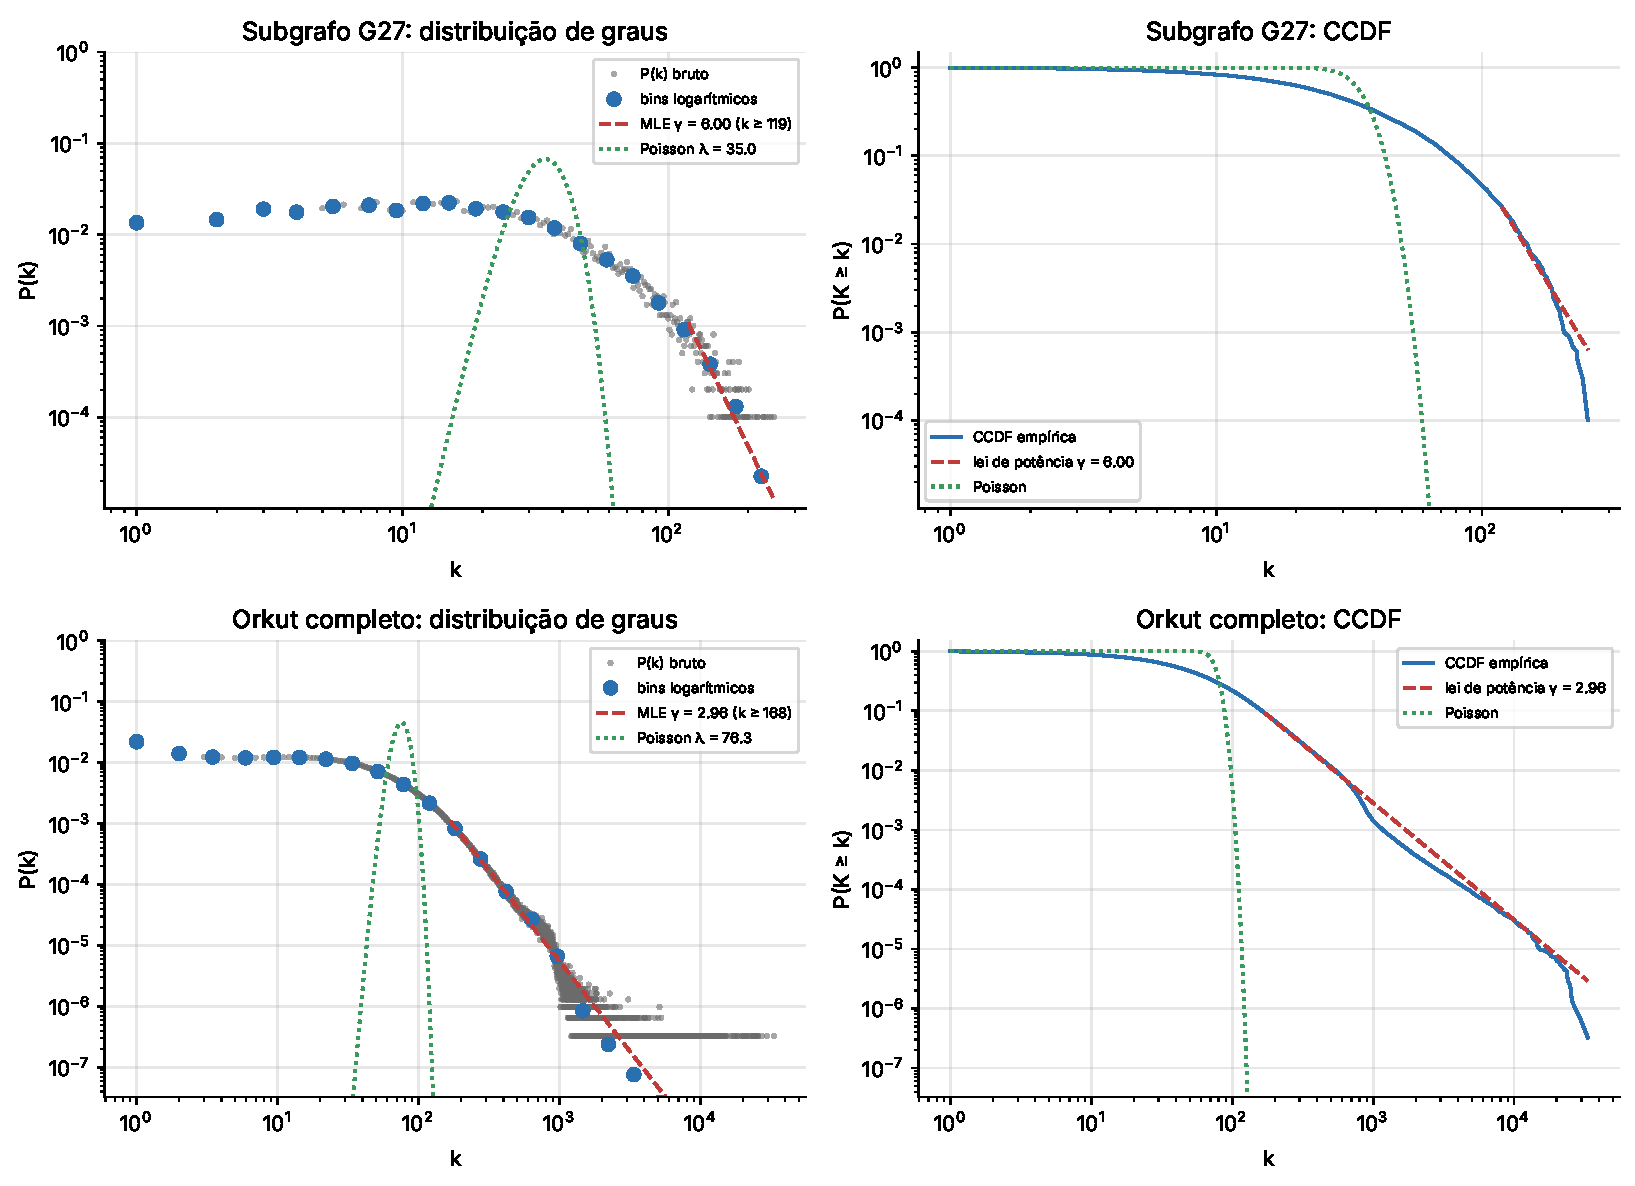
\includegraphics[width=0.92\textwidth]{figuras/p3_lei_potencia.pdf}
\caption{Lei de potência no subgrafo (linha superior) e no Orkut completo (linha inferior). Esquerda: $P(k)$ bruto (cinza), em bins logarítmicos (azul), ajuste MLE para $k \geq k_{\min}$ (vermelho) e Poisson com $\lambda = \langle k \rangle$ (verde). Direita: CCDF empírica, lei de potência ajustada e Poisson.}
\label{fig:powerlaw}
\end{figure*}

\begin{table*}[!htb]
\centering
\caption{Estimativas do expoente de $P(k) \sim C k^{-\gamma}$ no subgrafo e no Orkut completo.}
\label{tab:powerlaw}
\begin{adjustbox}{max width=\linewidth}
\begin{tabular}{lcc}
\toprule
Método & Subgrafo G27 & Orkut completo \\
\midrule
Regressão log-log, pontos brutos: γ (R²) & 1,61 (0,74) & 2,13 (0,84) \\
Regressão log-log, bins logarítmicos: γ (R²) & 0,94 (0,57) & 1,92 (0,89) \\
Regressão na CCDF: γ = 1 − inclinação (R²) & 2,85 (0,74) & 2,93 (0,97) \\
MLE discreta: γ ± erro-padrão & 6,00 ± 0,31 & 2,96 ± 0,004 \\
k\_min (mínima distância KS) / vértices na cauda & 119 / 259 & 168 / 289.226 \\
Distância KS na cauda & 0,057 & 0,016 \\
Vuong vs. exponencial: z (p) & -2,91 (0,0036) & 33,9 (< 1e-200) \\
Modelo favorecido na cauda & exponencial & lei de potência \\
KS global da Poisson (λ = grau médio) & 0,44 & 0,58 \\
\bottomrule
\end{tabular}
\end{adjustbox}
\end{table*}


\begin{figure}[!htb]
\centering
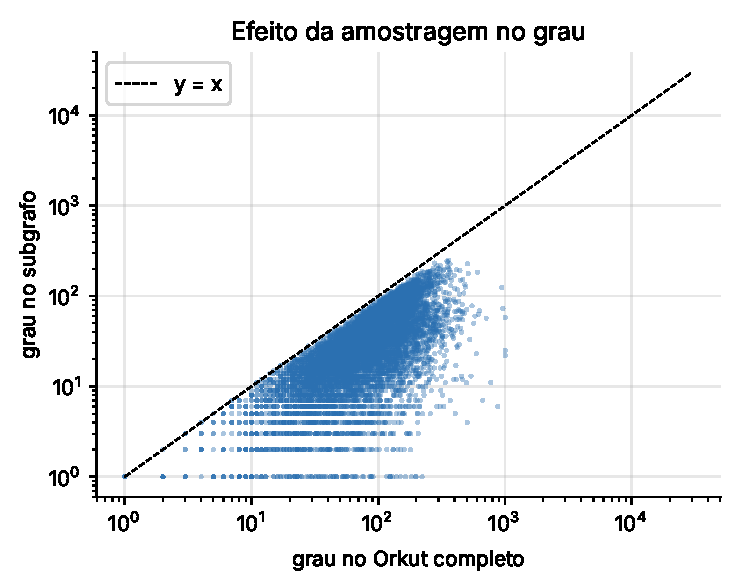
\includegraphics[width=0.75\linewidth]{figuras/p3_grau_original_vs_subgrafo.pdf}
\caption{Grau no Orkut completo $\times$ grau no subgrafo (log-log); tracejado: $y = x$.}
\label{fig:grauorig}
\end{figure}

\subsubsection{A rede é robusta?}
\textbf{Sim, tanto a falhas aleatórias quanto a ataques por grau. É moderadamente vulnerável a ataques por betweenness.} A Tabela~\ref{tab:robustez} e a Figura~\ref{fig:rob} comparam as estratégias. Com \robR{} vértices removidos ao acaso, a maior componente mantém $S = \robSaleat$ dos vértices restantes (IC95 [\robSaleatInf; \robSaleatSup], Tabela~\ref{tab:robustezic}), formam-se em média \robCaleat{} componentes (só vértices isolados) e $L$ sobe \robLaumAleat\%. O ataque aos de maior grau é quase igual: $S = \robSgrau$, $c = \robCgrau$, dentro da variação aleatória. Ele só alonga mais os caminhos ($L = \robLgrau$, $+\robLaumGrau\%$; $E$ cai de \robEbase{} para \robEgrau). O ataque por betweenness é o mais danoso: $S = \robSbet$, \robCbet{} componentes (\robCbetRazao{} vezes a média aleatória), $L = \robLbet$ ($+\robLaumBet\%$) e $E = \robEbet$. O PageRank fica entre os dois. A Figura~\ref{fig:curvas} estende a remoção até 50\%. Nas três estratégias, a maior componente encolhe quase só pelos vértices removidos (as curvas de $S$ ficam próximas da reta $1 - f$), mas os ataques, principalmente por betweenness, separam mais componentes desde o início.

Esse comportamento é o contrário do esperado para uma rede livre de escala ideal~\cite{albert2000}, em que o ataque aos hubs é devastador. Aqui os hubs estão no núcleo denso das comunidades, onde há muitos caminhos alternativos (5\% dos vértices de maior grau tocam \topCincoPct\% das arestas, mas quase todas as arestas deles são redundantes). Os vértices críticos são os que ligam comunidades. % INTERPRETAÇÃO

\begin{table}[!htb]
\centering
\caption{Robustez: remoção de $r = \lceil 0{,}05 n\rceil = 496$ vértices. Aleatória: média de 30 repetições; ataques: ranking fixo calculado no grafo intacto. $L$ e $E$ estimados com 200 fontes.}
\label{tab:robustez}
\begin{adjustbox}{max width=\linewidth}
\begin{tabular}{lrrrr}
\toprule
Estratégia & S (fração na LCC) & c (componentes) & L (caminho médio) & E (eficiência) \\
\midrule
Sem remoção & 1,0000 & 1,0 & 3,778 & 0,2799 \\
Aleatória (média de 30) & 0,9992 & 7,8 & 3,796 & 0,2784 \\
Ataque: Grau & 0,9990 & 8,0 & 4,025 & 0,2620 \\
Ataque: Betweenness & 0,9960 & 36,0 & 4,246 & 0,2471 \\
Ataque: PageRank & 0,9976 & 22,0 & 4,147 & 0,2552 \\
\bottomrule
\end{tabular}
\end{adjustbox}
\end{table}

\begin{table}[!htb]
\centering
\caption{Remoção aleatória: média, desvio-padrão e IC de 95\% (Normal, $n = 30$).}
\label{tab:robustezic}
\begin{adjustbox}{max width=\linewidth}
\begin{tabular}{lrrrr}
\toprule
Métrica & Média & DP & IC95 inf. & IC95 sup. \\
\midrule
S & 0,9992 & 0,0004 & 0,9991 & 0,9993 \\
c & 7,8333 & 2,8658 & 6,8078 & 8,8588 \\
L & 3,7960 & 0,0285 & 3,7858 & 3,8062 \\
E & 0,2784 & 0,0022 & 0,2776 & 0,2792 \\
\bottomrule
\end{tabular}
\end{adjustbox}
\end{table}


\begin{figure*}[!htb]
\centering
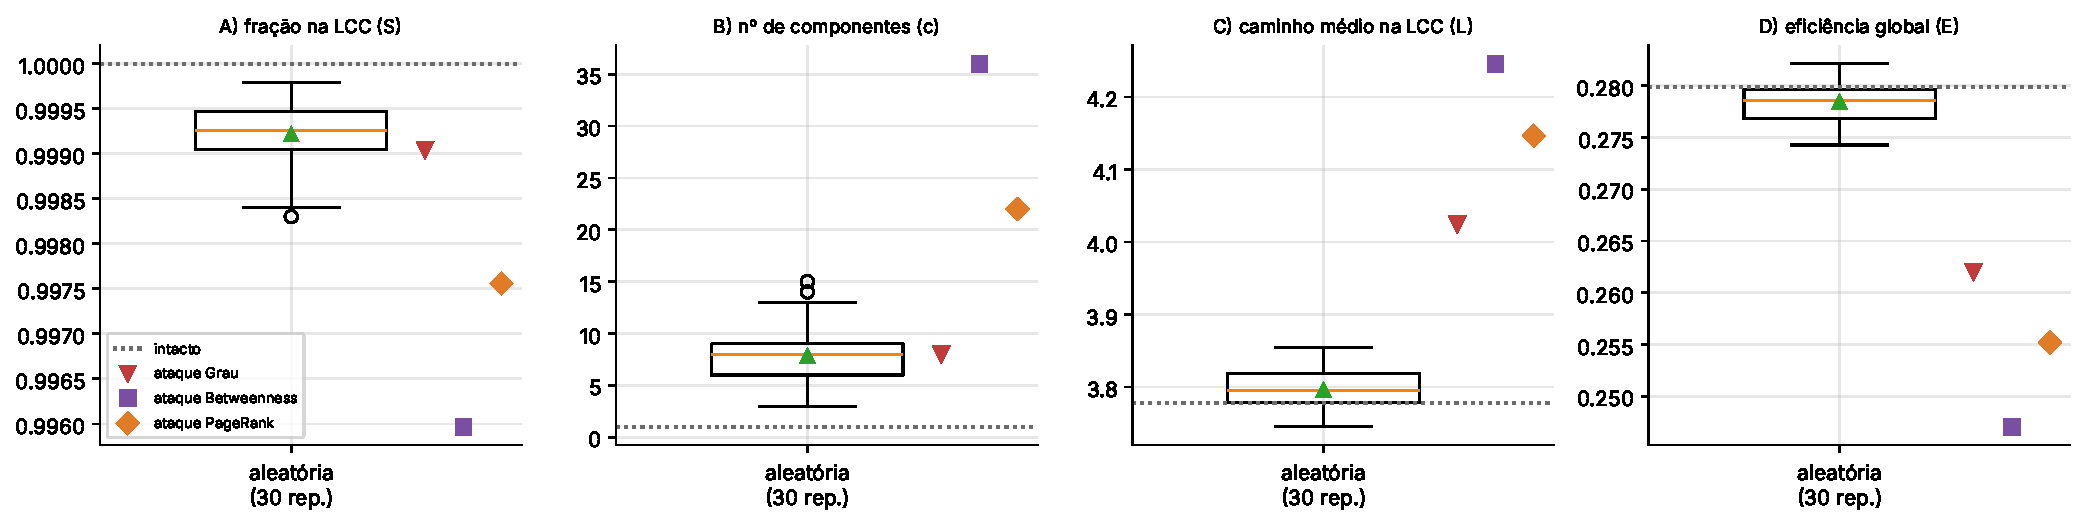
\includegraphics[width=\textwidth]{figuras/p3_robustez_5pct.pdf}
\caption{Robustez com $r = \robR$ (5\%): distribuição das 30 remoções aleatórias (boxplot; triângulo = média) e valor de cada ataque (grau, betweenness, PageRank) para as métricas A--D. Linha pontilhada: grafo intacto.}
\label{fig:rob}
\end{figure*}

\begin{figure*}[!htb]
\centering
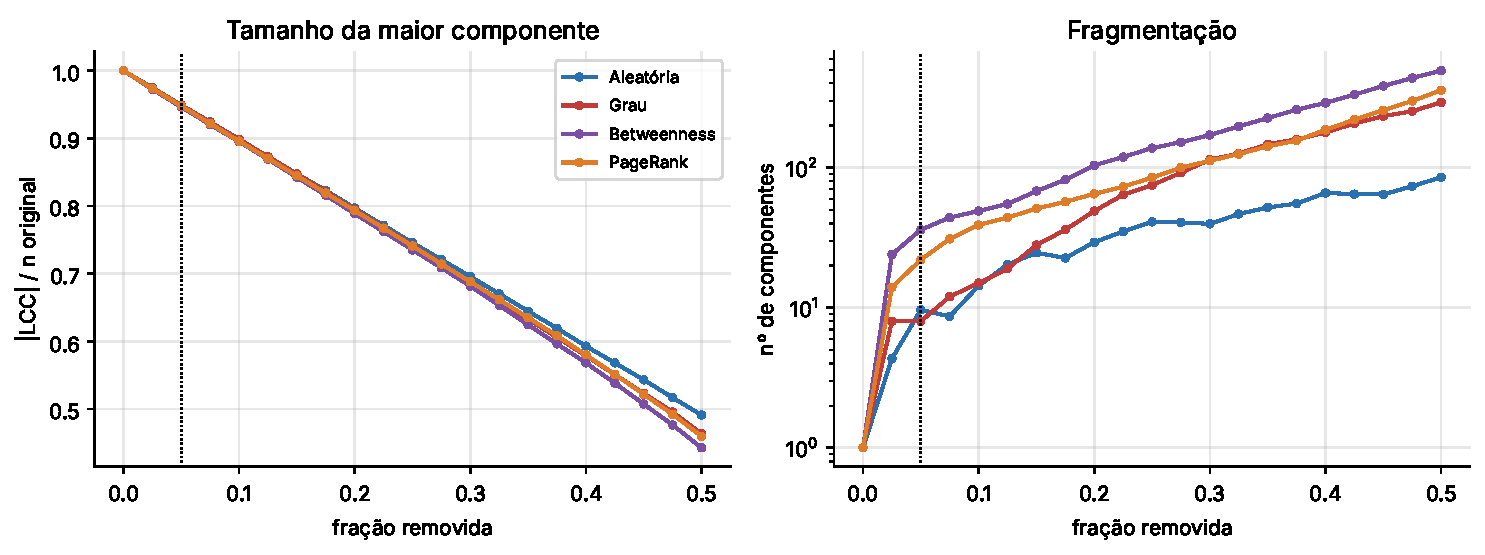
\includegraphics[width=0.85\textwidth]{figuras/p3_robustez_curvas.pdf}
\caption{Tamanho da maior componente (fração do $n$ original) e número de componentes (escala log) em função da fração removida; aleatória = média de 3 repetições. Linha pontilhada: 5\%.}
\label{fig:curvas}
\end{figure*}

\subsubsection{Qual foi a descoberta mais interessante?}
\textbf{Quem sustenta esta região do Orkut não são os hubs, e sim os vértices-ponte entre comunidades.} Quatro resultados independentes apontam na mesma direção. % INTERPRETAÇÃO — reescrever com suas palavras
(i) \fracIntraComunidade\% das arestas ligam usuários que compartilham pelo menos uma comunidade, e a clusterização é \swGammaConf{} vezes maior que a de um aleatório com os mesmos graus: a estrutura vem das comunidades, não da distribuição de graus.
(ii) A Tabela~\ref{tab:hubs} mostra que os 10 maiores hubs têm betweenness baixa e clusterização local de 0,16 a 0,27, ou seja, estão dentro de grupos densos. As exceções são os vértices 177048 (clusterização 0,056) e 24553 (5 comunidades), com betweenness de 7 a 11 vezes a mediana dos outros hubs.
(iii) Os \fracMultiCom\% de vértices que pertencem a duas ou mais comunidades têm betweenness média \betRazaoCom{} vezes maior (Figura~\ref{fig:descoberta}, direita; Spearman entre nº de comunidades e betweenness $= \spComBet$). São eles que o ataque por betweenness remove, e por isso ele fragmenta a rede \robCbetRazao{} vezes mais que o acaso, enquanto o ataque por grau não se distingue do acaso.
(iv) A clusterização cai pouco com o grau ($C(k) \sim k^{-\ckExpoente}$, $R^2 = \ckRdois$; Figura~\ref{fig:descoberta}, esquerda), longe do $k^{-1}$ de redes hierárquicas~\cite{ravasz2003}: hubs e vértices comuns estão igualmente imersos em grupos.
Na prática, para conectar ou desconectar grupos no Orkut, o que importa são as pessoas que transitam entre comunidades, e não as mais populares, em linha com os laços fracos de \citet{granovetter1973}. Uma segunda descoberta, metodológica, é que a lei de potência do Orkut ($\gamma \approx \plGammaFull$) não sobrevive à amostragem por comunidades, embora $C$ e $L$ sobrevivam.

\begin{table*}[!htb]
\centering
\caption{Os 10 vértices de maior grau no subgrafo (betweenness normalizada, estimada com 1.000 fontes).}
\label{tab:hubs}
\begin{adjustbox}{max width=\linewidth}
\begin{tabular}{lrrrrrr}
\toprule
id Orkut & grau (subgrafo) & grau (Orkut completo) & betweenness & PageRank & clusterização local & nº comunidades \\
\midrule
378358 & 250 & 358 & 0,0025 & 0,00036 & 0,214 & 2 \\
94761 & 243 & 349 & 0,0023 & 0,00038 & 0,164 & 2 \\
171264 & 239 & 355 & 0,0016 & 0,00034 & 0,234 & 3 \\
98891 & 232 & 278 & 0,0012 & 0,00035 & 0,242 & 2 \\
96420 & 228 & 507 & 0,0042 & 0,00038 & 0,174 & 1 \\
12173 & 227 & 369 & 0,0017 & 0,00033 & 0,256 & 3 \\
499180 & 218 & 309 & 0,0009 & 0,00031 & 0,267 & 3 \\
177048 & 216 & 291 & 0,0178 & 0,00076 & 0,056 & 1 \\
246019 & 211 & 354 & 0,0007 & 0,00030 & 0,266 & 4 \\
24553 & 203 & 299 & 0,0111 & 0,00037 & 0,181 & 5 \\
\bottomrule
\end{tabular}
\end{adjustbox}
\end{table*}


\begin{figure*}[!htb]
\centering
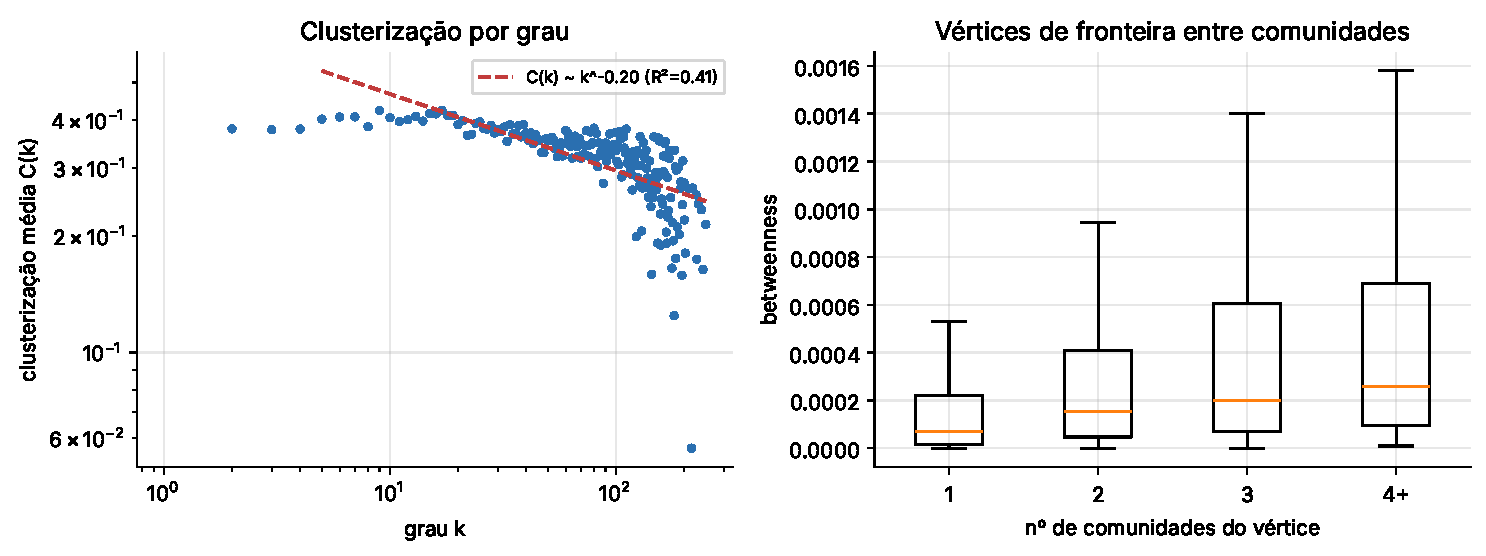
\includegraphics[width=0.85\textwidth]{figuras/p3_descoberta.pdf}
\caption{Esquerda: clusterização média $C(k)$ por grau (log-log) e ajuste para $k \geq 5$. Direita: betweenness por número de comunidades a que o vértice pertence (boxplot sem \emph{outliers}).}
\label{fig:descoberta}
\end{figure*}

\subsubsection{Extra: comparação com modelos clássicos}
A Tabela~\ref{tab:modelos} e a Figura~\ref{fig:modelos} comparam o Orkut G27 com geradores próprios de Erdős–Rényi~\cite{erdos1959}, Barabási–Albert~\cite{barabasi1999} ($m_0 = 17$) e Watts–Strogatz~\cite{watts1998} ($k = 34$, $p = 0{,}1$), todos com $n = \nV$ e $m$ aproximado. Nenhum modelo reproduz as três propriedades ao mesmo tempo. O ER tem $L$ curto, mas $C$ cem vezes menor e graus concentrados (máximo \erGrauMax). O BA gera cauda de potência ($\gamma = \baGamma$, grau máximo \baGrauMax), mas $C = \baC$. O WS reproduz $C$ alto (\wsC) e $L$ curto (\wsL), mas tem graus quase constantes (máximo \wsGrauMax). A CCDF do Orkut G27 fica entre a do ER e a do BA: mais heterogênea que a Poisson, sem chegar à cauda do BA. Ela se aproximaria do BA no grafo completo, cujo $\gamma \approx 3$ é o do modelo. O Orkut combina a clusterização do WS com uma heterogeneidade de graus intermediária, e o que falta aos três modelos é justamente a estrutura comunitária sobreposta. % INTERPRETAÇÃO

\begin{table*}[!htb]
\centering
\caption{Orkut G27 contra modelos clássicos gerados com o mesmo $n$ e $m$ aproximado. $L$ dos modelos estimado com 500 fontes; γ e $k_{\min}$ pela MLE discreta; última coluna: teste de Vuong na cauda.}
\label{tab:modelos}
\begin{adjustbox}{max width=\linewidth}
\begin{tabular}{lrrrrrrrrr}
\toprule
Modelo & n & m & grau médio & grau máx. & C & L & γ MLE & k\_min & cauda (Vuong) \\
\midrule
Orkut G27 & 9.917 & 173.413 & 34,97 & 250 & 0,3703 & 3,764 & 6,00 & 119 & exponencial \\
Erdős–Rényi & 9.917 & 173.413 & 34,97 & 59 & 0,0035 & 2,896 & 19,77 & 47 & exponencial \\
Barabási–Albert (m=17) & 9.917 & 168.436 & 33,97 & 568 & 0,0171 & 2,807 & 2,93 & 21 & potência \\
Watts–Strogatz (k=34, p=0,1) & 9.917 & 168.589 & 34,00 & 41 & 0,5307 & 3,597 & 20,00 & 34 & exponencial \\
\bottomrule
\end{tabular}
\end{adjustbox}
\end{table*}


\begin{figure}[!htb]
\centering
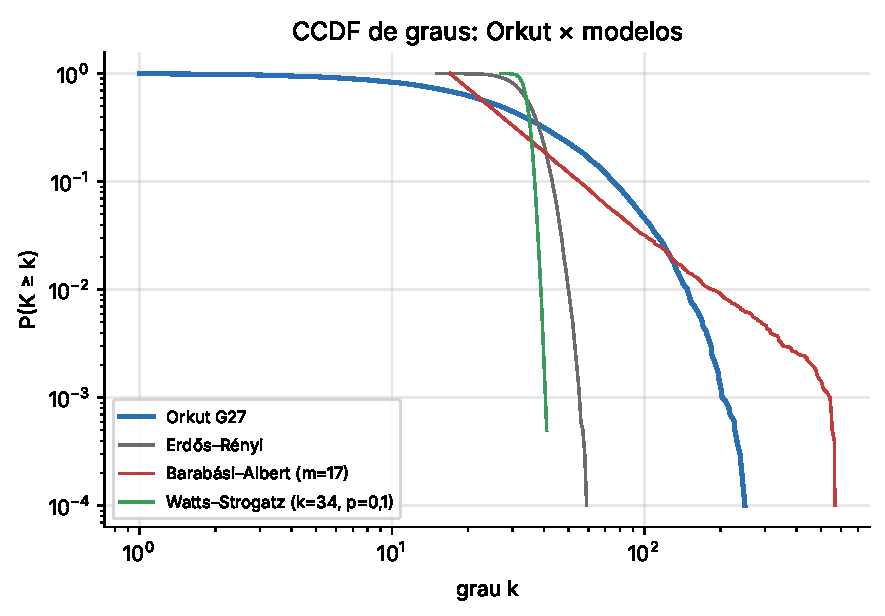
\includegraphics[width=0.9\linewidth]{figuras/p3_modelos_ccdf.pdf}
\caption{CCDF de graus (log-log) do Orkut G27 e dos modelos ER, BA e WS com mesmos $n$ e $m$ aproximado.}
\label{fig:modelos}
\end{figure}

% =====================================================================
\section{Discussão crítica}\label{sec:discussao}
\paragraph{Tratamento.} O subgrafo é uma região coesa do Orkut, não uma amostra representativa da rede inteira. Por construção, isso favorece clusterização alta, conectividade e robustez, e corta a cauda de graus (Figura~\ref{fig:grauorig}). As conclusões sobre \emph{small-world}, robustez e descoberta valem para regiões comunitárias do Orkut. A da lei de potência foi tirada do grafo completo justamente por esse motivo. Outra semente, ou uma expansão BFS/\emph{snowball}, produziria outro subgrafo; não medimos a variabilidade entre sementes.

\paragraph{Aproximações.} As medidas da Parte~I são exatas. Já $L$ dos modelos nulos (1.000 fontes), $L$ e $E$ na robustez (200 fontes) e o betweenness (1.000 fontes) são estimativas. O desvio-padrão de $L_r$ entre instâncias ER foi da ordem de $10^{-3}$, e o $L$ do grafo intacto estimado com 200 fontes (\robLbase) difere do exato (\caminhoMedio) em 0,4\%, o que basta para as comparações feitas. Os modelos nulos usaram poucas instâncias (5 e 3).

\paragraph{Pesos.} O peso de \emph{embeddedness} é uma escolha nossa, derivada da topologia, e não um dado do SNAP. Ele dá sentido a Dijkstra, Bellman-Ford, Floyd-Warshall e à árvore geradora mínima, mas não representa intensidade de interação real.

\paragraph{Testes que faltaram.} Não testamos a lei de potência contra a lognormal (alternativa comum para redes sociais) nem estimamos o p-valor da lei de potência por \emph{bootstrap}~\cite{clauset2009}. A robustez usou ranking fixo, sem recalcular a centralidade após cada remoção (ataque adaptativo), o que tenderia a ser ainda mais danoso.

\paragraph{Dependência de máquina.} Os tempos absolutos dependem do processador, do Python e da carga do sistema. O que se transfere para outras máquinas são as razões entre algoritmos e os expoentes de crescimento. As medições foram feitas no ambiente indicado na Seção~\ref{sec:metodo}.

\paragraph{Origem dos dados.} A rede é de 2006--2007 e foi obtida por \emph{crawling}~\cite{mislove2007}, o que pode sub-representar usuários pouco conectados. As comunidades são grupos declarados pelos usuários, não comunidades detectadas por algoritmo.

% =====================================================================
\section{Conclusão}
Analisamos o grafo G27 (com-Orkut) a partir de uma auditoria completa do arquivo bruto e de uma redução por comunidades que preserva a estrutura local. A LCC de \nV{} vértices é esparsa, mas muito agrupada ($C = \clusterMedia$), e tem caminhos curtos ($L = \caminhoMedio$, diâmetro \diametro). Implementamos e validamos os nove algoritmos da Parte~II; seus tempos acompanham a complexidade teórica. A rede é \emph{small-world} contra os dois nulos. O Orkut completo segue uma lei de potência com $\gamma \approx \plGammaFull$, que a amostragem apaga. A rede resiste a falhas e a ataques por grau, mas é mais sensível à remoção de quem liga comunidades, e essa é a descoberta central do trabalho. Como trabalhos futuros, propomos repetir a análise com várias sementes e com amostragem BFS/\emph{snowball}, testar ataques adaptativos, comparar a cauda com a lognormal e usar algoritmos de detecção de comunidades para verificar se os vértices de alta betweenness coincidem com as fronteiras detectadas.

\bibliographystyle{ACM-Reference-Format}
\bibliography{referencias}

\end{document}
